\section{Operating Data}

%%%%%%%%%%%%%%%%%%%%%%%%%%%%%%%%%%%%%%%%%%%%%%%%%%%%%%%%%%%%%%%%%%%%%%%%%%%%%%%%
\subsection{Processing Measured In-Core Detector Data}
\label{sec:process_measure}
In this reactor plant, there are 58 assemblies that contain in-core detectors.
This layout of in-core detectors is shown in Figure \ref{fig_instr_pos}. These
detectors are typically U-235 fission chambers varying in mass of U-235.
Although there are 58 locations, there are usually only a few detectors (6-10).
When measurements are being taken, multiple \textit{passes} are performed to
adequately measure all 58 assemblies. Each detector will, however, pass through
one common assembly. This becomes important in the normalization process of
detector signals.

Before a measurement is taken, detectors are inserted into the core through 
instrumentation tubes in assemblies until the top of the assembly is hit.
Detector measurements are then taken as the detectors are pulled back through
the core at a constant speed. Thus, each measurement reported is an integral of
the signal over the recording time. Also, axial locations of where data is
recorded may be slightly skewed. In these measurements, 61 axial data points
were collected and processed with a Python script.

%%%%%%%%%%%%%%%%%%%%%%%%%%%%%%%%%%%%%%%%%%%%%%%%%%%%%%%%%%%%%%%%%%%%%%%%%%%%%%%%
\subsubsection{Example -- Hot Zero Power Measurements}

This section will go through the process of filtering measured data for
\ac{HZP}.  It should be noted that the algorithm developed to process \ac{HZP}
data was used for all detector data. Therefore, some of the detector maps may
show errors in processing. Current work is underway to develop an algorithm
that can be applied to all data. Under \ac{HZP} conditions, the core power for
these measurements is approximately 25 MWth.  Raw data was processed by first
organizing it in Python objects. Each collection of measurements contain
detector information for multiple passes through the core in various assemblies.
Raw data for \ac{HZP} is shown in Figure \ref{fig:orig_all}. In order to show
all detector signals on one plot, each raw data signal was normalized to a sum
of unity.
\begin{figure}
    \centering
    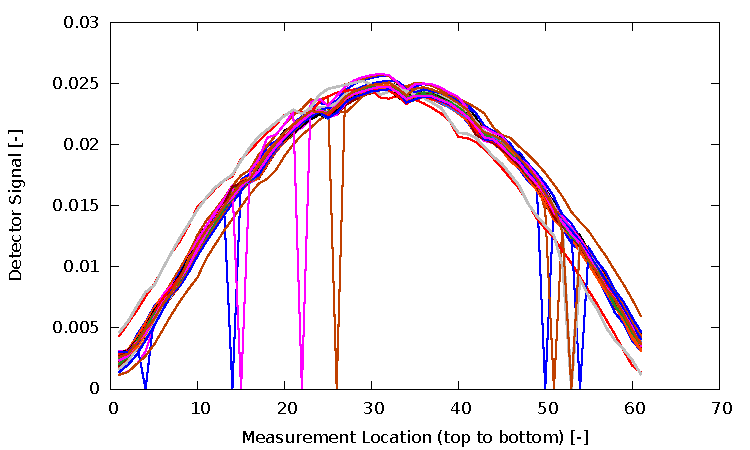
\includegraphics{expdata/figs/original_all.pdf}
    \caption{Initial Raw Detector Measurements (top to bottom). \label{fig:orig_all}}
\end{figure}

The first step in this process is to remove any detector background signal. This 
information was supplied with the raw data and can be subtracted from each 
detector measurement pass. The corrected data for background is shown in Figure 
\ref{fig:back_all}.
\begin{figure}
    \centering
    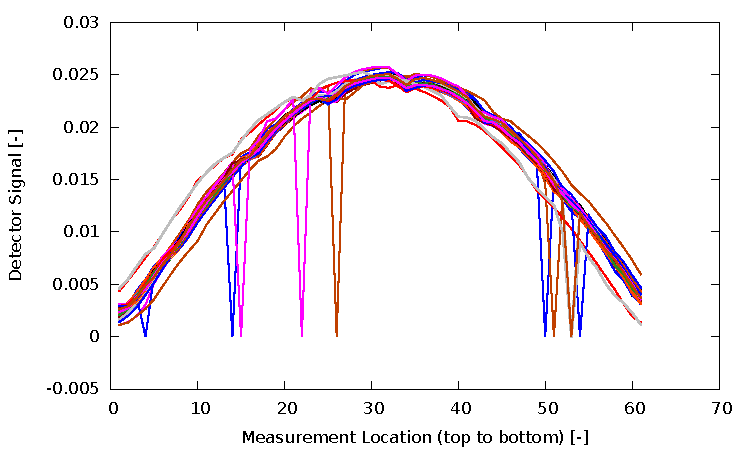
\includegraphics{expdata/figs/background_all.pdf}
    \caption{Detector Measurements Corrected for Background (top to bottom). \label{fig:back_all}}
\end{figure}

Depending on the strength of the signal being measured, the signal can be amplified
by adjusting the gain on the detectors.  Gain factors are also reported with the raw data.  When 
processing, these gain factors are multiplied by the measured data.  For \ac{HZP}, all 
of the gain factors are unity.  Figure \ref{fig:gain_all} shows the measured data 
after gain factors are applied.
\begin{figure}
    \centering
    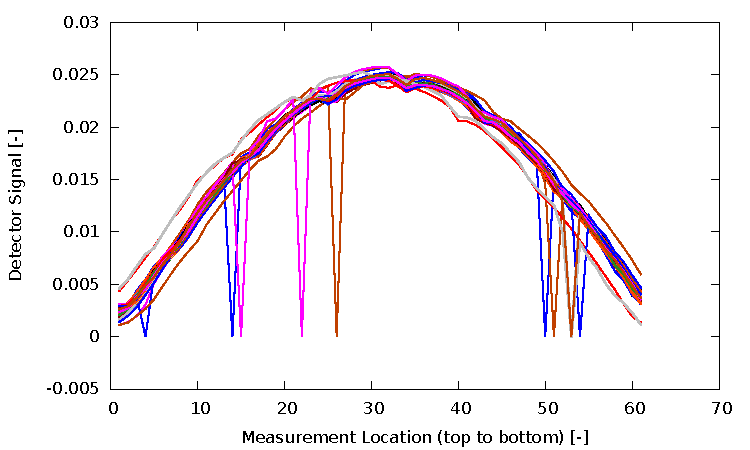
\includegraphics{expdata/figs/gain_all.pdf}
    \caption{Detector Measurements Gain Factors Applied (top to bottom). \label{fig:gain_all}}
\end{figure}

In some of the detector signals, zero points exist where the detector failed.  These zero points are removed by performing
a linear interpolation/extrapolation between/from the nearest two points.  The corrected data is shown 
in Figure \ref{fig:zero}.
\begin{figure}
    \centering
    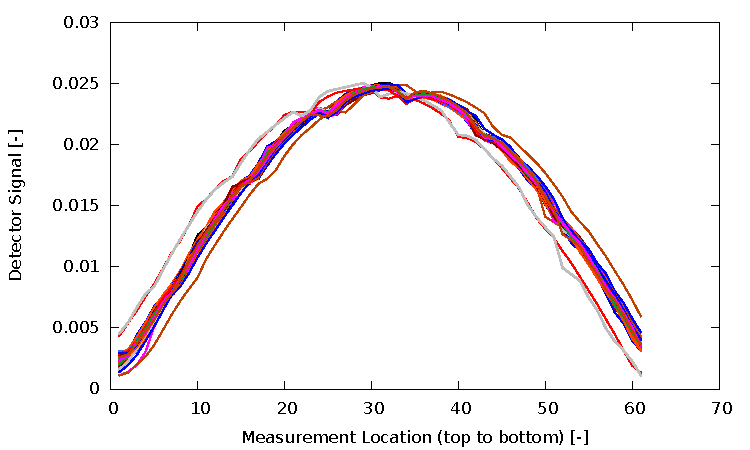
\includegraphics{expdata/figs/zeros_all.pdf}
    \caption{Detector Measurements with Zero Points Removed (top to bottom). \label{fig:zero}}
\end{figure}

As explained above, there is one common assembly where all detectors will pass. This is needed 
for normalization of detector signals. In this plant, assembly J10 was chosen as the common
assembly.  Figure \ref{fig:J10} shows the measurements taken in assembly J10.
\begin{figure}
    \centering
    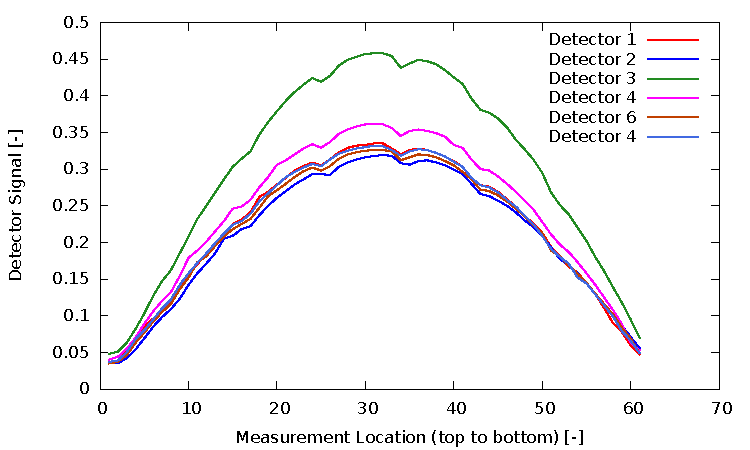
\includegraphics{expdata/figs/zeros.pdf}
    \caption{Detector Measurements with in J10 Assembly (top to bottom). \label{fig:J10}}
\end{figure}

Each detector measurement represents a different measurement pass.  The core power
during one pass may not be the same as the others. There is typically a small fluctuation present in the core power. To account for this, each signal
is divided by the core power reported during that measurement pass. The resulting
detector signals are shown in Figure \ref{fig:dividepower} for assembly J10.
\begin{figure}[htbp]
    \centering
    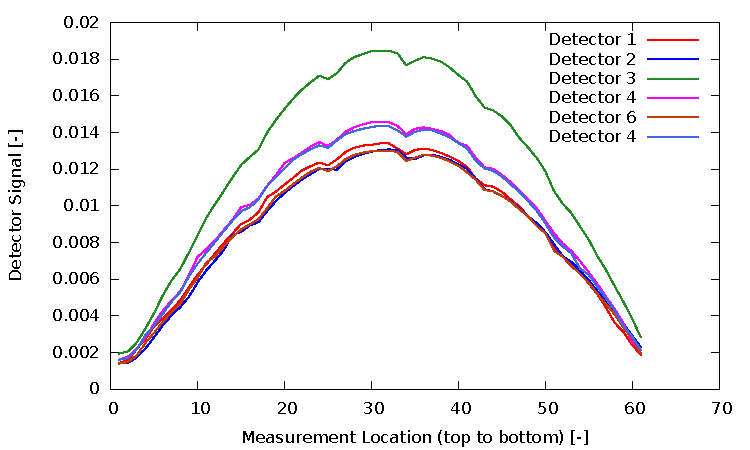
\includegraphics{expdata/figs/divide_power.pdf}
    \caption{J10 Detector Measurements Divided by Core Power (top to bottom). \label{fig:dividepower}}
\end{figure}

The next step in the process is to make sure that all detector signals line up with
one another. We can verify this by plotting all 58 detector signals on top of each 
other.  This is the same as plot as Figure \ref{fig:dividepower}, except all assemblies are plotted here with signals normalized for shape comparison. This is shown in Figure \ref{fig:beforerealign}.
\begin{figure}[htbp]
    \centering
    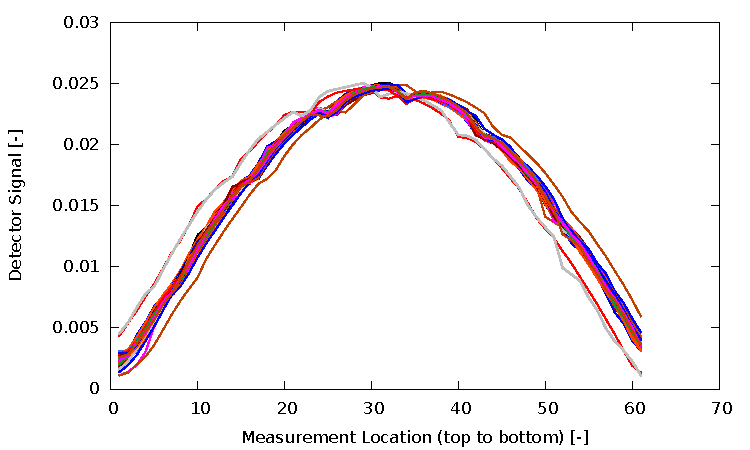
\includegraphics{expdata/figs/before_realign.pdf}
    \caption{All Detector Signals Before Realignment. \label{fig:beforerealign}}
\end{figure}
It is observed that not all of the signals are aligned with each other. Luckily, signals can be 
aligned to grid depressions. Here, we align to three grid depression positions, 25, 34, and 42, which are located in the centerline of grid 5, grid 4 and grid 3 respectively.
The first step in this process is to find the measurement indexes corresponding to the local minimum in three regions, 22 to 28, 31 to 37, and 39 to 45 respectively.
Then for each assembly, if the measurement indexes are inconsistent with correct indexes,
a shifting length is estimated to make all the measurement indexes best match the correct indexes.
All grids are then shifted either left or right. Depending on the 
shift direction, one end will lose a point and the other will gain one. The data point 
that is lost is just deleted from the data array, while the point that is gained is 
determined by a simple linear extrapolation from the nearest two points. The resulting 
realignment is shown in Figure \ref{fig:afterrealign}.
\begin{figure}[htbp]
    \centering
    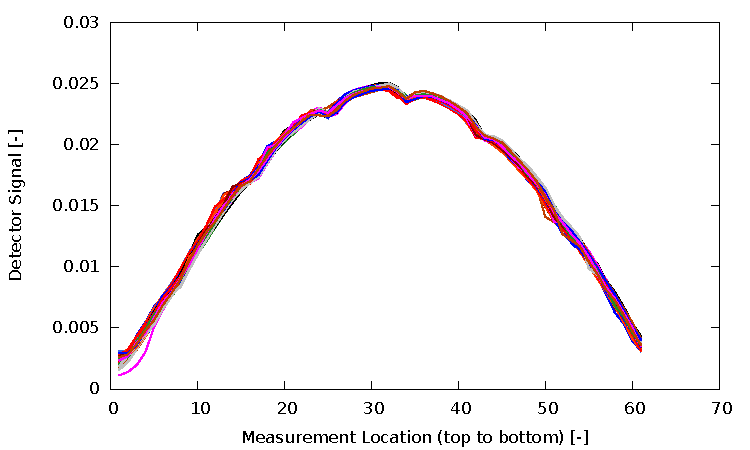
\includegraphics{expdata/figs/after_realign.pdf}
    \caption{All Detector Signals After Realignment. \label{fig:afterrealign}}
\end{figure}
Results show that all detector signals are more consistently aligned, however still not perfect. The span of these signals can also be attributed to measurement uncertainty as they should all have the same shape once normalized here. There 
is one signal that is an outlier is observed between measurements 
0 and 5. This assembly location corresponds to where control rod bank D 
is slightly inserted. Therefore, we should expect this depression in the signal toward 
the top of the core.

The next step in the process is to average detector signals that were measured from
the same detector. It is important to look at the raw signals before performing this
step since measurements may be poor. If this is observed, the poor measurement
is commented out in the data file. In Figure \ref{fig:dividepower} the two signals
from detector 4 are close to each other and should be averaged. The resulting signals
for assembly J10 are shown in Figure \ref{fig:averagemultiple}.
\begin{figure}[htbp]
    \centering
    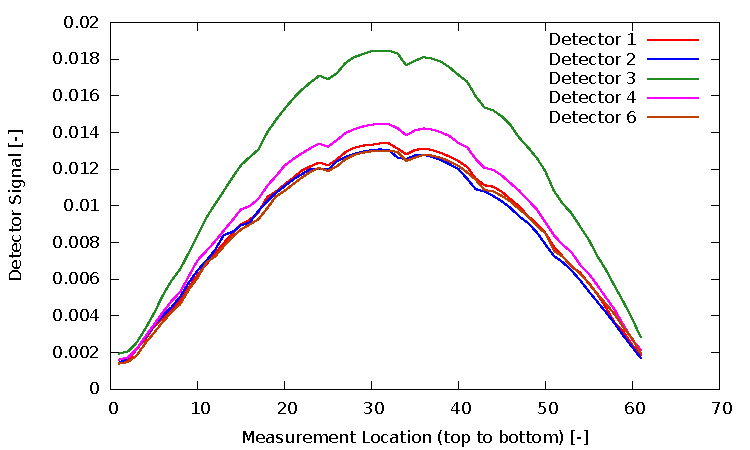
\includegraphics{expdata/figs/average_multiple.pdf}
    \caption{Multiple Detector Signals Averaged in J10 (top to bottom). \label{fig:averagemultiple}}
\end{figure}

Each fission chamber detector contains a different amount of U-235. Therefore, some normalization 
process is needed to account for this mass difference. To get these normalization factors,
the average of all detector signals is determined first. Then, normalization factors
are computed by taking the ratio of the integral of each individual detector signal
to the integral of the mean of all detector signals. For example, for \ac{HZP} the 
normalization factors for each detector are:
\begin{itemize}
  \item{Detector 1: 0.922}
  \item{Detector 2: 0.901}
  \item{Detector 3: 1.272}
  \item{Detector 4: 1.002}
  \item{Detector 6: 0.903}
\end{itemize}
These normalization factors are then multiplied to each corresponding detector signal 
in the core. The resulting signals are now very close to each other as shown in
Figure \ref{fig:detnorm} for assembly J10.
\begin{figure}[htbp]
    \centering
    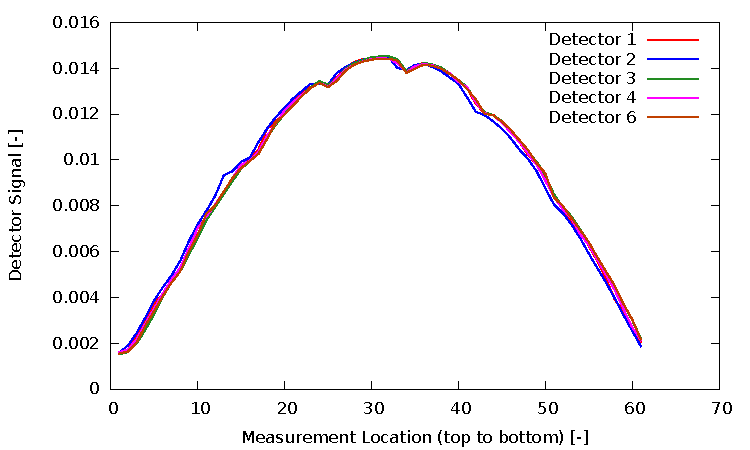
\includegraphics{expdata/figs/norm_factors.pdf}
    \caption{Application of Detector Normalization Factors for J10. \label{fig:detnorm}}
\end{figure}

Lastly, detector signals need to be put on an axial coordinate grid corresponding 
to points that range from the bottom to top of active fuel. To do this we use the same 
grid point as before since we know that the centerline location of this grid is at 
221.9 cm above bottom of active fuel. The distance between axial measurement locations 
is assumed uniform and is equal to active core height divided by 60 intervals. A 2nd 
order spline fit is then used to map from measured data axial locations to a axial map 
has equal data points exactly at the \ac{TAF} and \ac{BAF}.  A comparison of 
applying this spline is shown in Figure \ref{fig:splineassy}.
\begin{figure}[htbp]
    \centering
    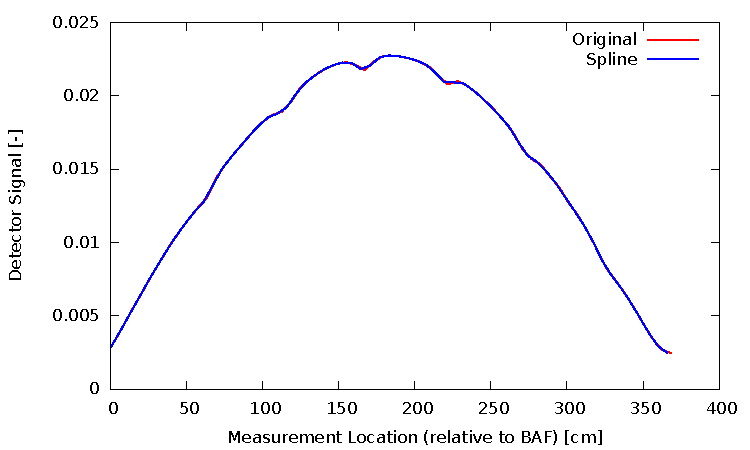
\includegraphics{expdata/figs/spline_assy.pdf}
    \caption{Comparison of Splined Data for Assembly J10. \label{fig:splineassy}}
\end{figure}
The spline fit does well for this data, however grid depressions are now less since the 
grid centerline does not match up with the final axial grid.  Before the spline, all 
detector signals were averaged such that there is only one signal per assembly. All splined 
signals are shown in Figure \ref{fig:splineall}. There is some spread in the data when they 
are all normalized to one another. There is one detector signal that seems to not follow the 
same shape at the top of the core. That measurement corresponds to assembly D12 where control 
rod bank D is slightly inserted and thus there is a depression in the measurement signal.
\begin{figure}[htbp]
    \centering
    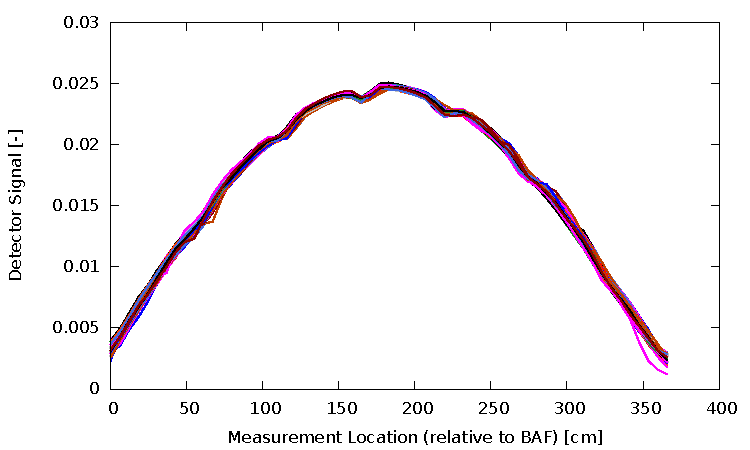
\includegraphics{expdata/figs/spline_all.pdf}
    \caption{Comparison of All Assemblies after Spline. \label{fig:splineall}}
\end{figure}
A separate Excel sheet contains all of the processed data organized by measurement 
data file and by assembly.  A plot of the final measurements (not all normalized to sum of unity) is 
shown in Figure \ref{fig:splineunnorm}.
\begin{figure}[htbp]
    \centering
    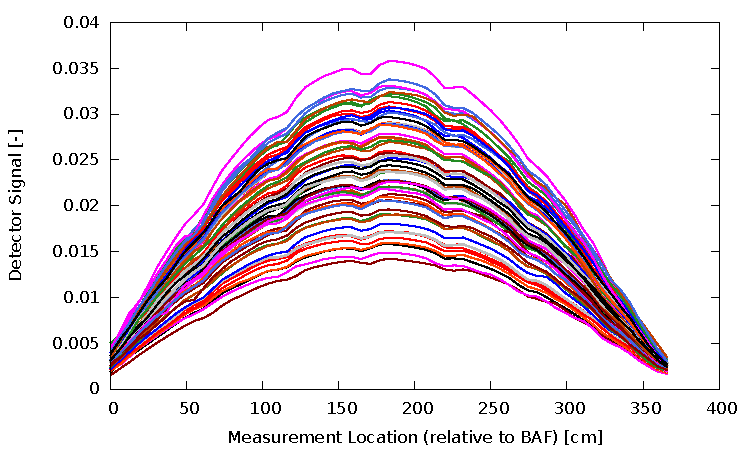
\includegraphics{expdata/figs/spline_unnorm.pdf}
    \caption{Final Processed \ac{HZP} Measurement Data. \label{fig:splineunnorm}}
\end{figure}

%%%%%%%%%%%%%%%%%%%%%%%%%%%%%%%%%%%%%%%%%%%%%%%%%%%%%%%%%%%%%%%%%%%%%%%%%%%%%%%%

\subsection{Hot Zero Power Data Discussion}
\label{sec:hzp_data_disc}

Table \ref{tbl:hzp_c1} lists the thermal power of the reactor during initial physics testing the first available detector maps. Also included are the rod bank positions and critical boron concentration. This data can be used to evaluate how far off reactor models are from critical at \ac{HZP} conditions.
\begin{table}[htp]
  \centering
  \caption{Cycle 1 hot zero power physics configuration.}
  \label{tbl:hzp_c1}
  \begin{tabular}{l r}
    \toprule
    Core Power & 25 MWth \\
    Core Flow Rate & $61.5\times10^6$ kg/hr \\ 
    Inlet Coolant Temperature & 560$^\circ$ F \\
    Rod Bank A Position & Step 228 \\
    Rod Bank B Position & Step 228 \\
    Rod Bank C Position & Step 228 \\
    Rod Bank D Position & Step 213 \\
    Boron Concentration & 975 \acs{ppm} \\
    \bottomrule
  \end{tabular}
\end{table}

Radial maps were also created to view the average relative power produced per assembly. 
These were obtained by renormalizing the signals in Figure \ref{fig:splineunnorm} such that their total
sum is the number of detector locations (in this case 58). Each measurement in an assembly was then 
axially averaged to produce a relative radial peaking factor. In Figure \ref{fig:radial_meas}, this factor 
is presented on each assembly where a measurement was taken.
\definecolor{Gsevencolor}{rgb}{1,1,1}
\definecolor{Gsixcolor}{rgb}{1,1,1}
\definecolor{Gfivecolor}{rgb}{0.8,0.618592167995,0.16}
\definecolor{Gfourcolor}{rgb}{1,1,1}
\definecolor{Gthreecolor}{rgb}{1,1,1}
\definecolor{Gtwocolor}{rgb}{1,1,1}
\definecolor{Gonecolor}{rgb}{1,1,1}
\definecolor{Gninecolor}{rgb}{0.8,0.784652300146,0.16}
\definecolor{Geightcolor}{rgb}{1,1,1}
\definecolor{Jeightcolor}{rgb}{0.454640153967,0.8,0.16}
\definecolor{Jninecolor}{rgb}{1,1,1}
\definecolor{Jfourcolor}{rgb}{1,1,1}
\definecolor{Jfivecolor}{rgb}{1,1,1}
\definecolor{Jsixcolor}{rgb}{1,1,1}
\definecolor{Jsevencolor}{rgb}{0.8,0.797530194246,0.16}
\definecolor{Jonecolor}{rgb}{0.459102226928,0.8,0.16}
\definecolor{Jtwocolor}{rgb}{1,1,1}
\definecolor{Jthreecolor}{rgb}{1,1,1}
\definecolor{Lfourteencolor}{rgb}{1,1,1}
\definecolor{Lfifteencolor}{rgb}{0.199325500465,0.8,0.16}
\definecolor{Ltencolor}{rgb}{0.736879753927,0.8,0.16}
\definecolor{Lelevencolor}{rgb}{0.8,0.418746058875,0.16}
\definecolor{Ltwelvecolor}{rgb}{1,1,1}
\definecolor{Lthirteencolor}{rgb}{0.8,0.306806119453,0.16}
\definecolor{Mfivecolor}{rgb}{1,1,1}
\definecolor{Mfourcolor}{rgb}{1,1,1}
\definecolor{Msevencolor}{rgb}{0.676919670852,0.8,0.16}
\definecolor{Msixcolor}{rgb}{1,1,1}
\definecolor{Mthreecolor}{rgb}{1,1,1}
\definecolor{Mtwocolor}{rgb}{1,1,1}
\definecolor{Mninecolor}{rgb}{1,1,1}
\definecolor{Meightcolor}{rgb}{1,1,1}
\definecolor{Ptencolor}{rgb}{1,1,1}
\definecolor{Pelevencolor}{rgb}{1,1,1}
\definecolor{Ptwelvecolor}{rgb}{1,1,1}
\definecolor{Pthirteencolor}{rgb}{1,1,1}
\definecolor{Peightcolor}{rgb}{1,1,1}
\definecolor{Pthreecolor}{rgb}{1,1,1}
\definecolor{Pninecolor}{rgb}{0.547691836697,0.8,0.16}
\definecolor{Psixcolor}{rgb}{1,1,1}
\definecolor{Psevencolor}{rgb}{1,1,1}
\definecolor{Pfourcolor}{rgb}{0.604342827129,0.8,0.16}
\definecolor{Pfivecolor}{rgb}{1,1,1}
\definecolor{Htencolor}{rgb}{1,1,1}
\definecolor{Helevencolor}{rgb}{0.743521203429,0.8,0.16}
\definecolor{Htwelvecolor}{rgb}{1,1,1}
\definecolor{Hthirteencolor}{rgb}{0.76691352318,0.8,0.16}
\definecolor{Hfourteencolor}{rgb}{1,1,1}
\definecolor{Hfifteencolor}{rgb}{0.548211017514,0.8,0.16}
\definecolor{Kthirteencolor}{rgb}{1,1,1}
\definecolor{Ktwelvecolor}{rgb}{0.8,0.478965220928,0.16}
\definecolor{Kelevencolor}{rgb}{1,1,1}
\definecolor{Ktencolor}{rgb}{1,1,1}
\definecolor{Dtencolor}{rgb}{0.8,0.378816128792,0.16}
\definecolor{Delevencolor}{rgb}{1,1,1}
\definecolor{Dtwelvecolor}{rgb}{0.8,0.16,0.16}
\definecolor{Dthirteencolor}{rgb}{1,1,1}
\definecolor{Cninecolor}{rgb}{1,1,1}
\definecolor{Ceightcolor}{rgb}{0.739353774059,0.8,0.16}
\definecolor{Cthreecolor}{rgb}{1,1,1}
\definecolor{Ctwocolor}{rgb}{1,1,1}
\definecolor{Csevencolor}{rgb}{0.8,0.507089861588,0.16}
\definecolor{Csixcolor}{rgb}{1,1,1}
\definecolor{Cfivecolor}{rgb}{0.8,0.333912008163,0.16}
\definecolor{Cfourcolor}{rgb}{1,1,1}
\definecolor{Heightcolor}{rgb}{1,1,1}
\definecolor{Nelevencolor}{rgb}{1,1,1}
\definecolor{Gfifteencolor}{rgb}{1,1,1}
\definecolor{Gfourteencolor}{rgb}{1,1,1}
\definecolor{Gthirteencolor}{rgb}{1,1,1}
\definecolor{Gtwelvecolor}{rgb}{0.8,0.759800445861,0.16}
\definecolor{Gelevencolor}{rgb}{1,1,1}
\definecolor{Gtencolor}{rgb}{1,1,1}
\definecolor{Fonecolor}{rgb}{0.343652135741,0.8,0.16}
\definecolor{Ftwocolor}{rgb}{1,1,1}
\definecolor{Fthreecolor}{rgb}{0.738726029798,0.8,0.16}
\definecolor{Ffourcolor}{rgb}{1,1,1}
\definecolor{Ffivecolor}{rgb}{1,1,1}
\definecolor{Fsixcolor}{rgb}{1,1,1}
\definecolor{Fsevencolor}{rgb}{0.629761330677,0.8,0.16}
\definecolor{Feightcolor}{rgb}{0.8,0.678403426852,0.16}
\definecolor{Fninecolor}{rgb}{1,1,1}
\definecolor{Cthirteencolor}{rgb}{1,1,1}
\definecolor{Ctwelvecolor}{rgb}{1,1,1}
\definecolor{Celevencolor}{rgb}{1,1,1}
\definecolor{Ctencolor}{rgb}{1,1,1}
\definecolor{Cfourteencolor}{rgb}{1,1,1}
\definecolor{Lsixcolor}{rgb}{1,1,1}
\definecolor{Lsevencolor}{rgb}{1,1,1}
\definecolor{Lfourcolor}{rgb}{1,1,1}
\definecolor{Lfivecolor}{rgb}{0.8,0.565450550792,0.16}
\definecolor{Ltwocolor}{rgb}{1,1,1}
\definecolor{Lthreecolor}{rgb}{1,1,1}
\definecolor{Lonecolor}{rgb}{1,1,1}
\definecolor{Leightcolor}{rgb}{0.667827761744,0.8,0.16}
\definecolor{Lninecolor}{rgb}{1,1,1}
\definecolor{Dfourteencolor}{rgb}{0.8,0.73524663764,0.16}
\definecolor{Kfifteencolor}{rgb}{1,1,1}
\definecolor{Kfourteencolor}{rgb}{1,1,1}
\definecolor{Rfivecolor}{rgb}{1,1,1}
\definecolor{Rsixcolor}{rgb}{0.300807032861,0.8,0.16}
\definecolor{Rsevencolor}{rgb}{1,1,1}
\definecolor{Reightcolor}{rgb}{0.389434761288,0.8,0.16}
\definecolor{Rninecolor}{rgb}{1,1,1}
\definecolor{Bfourcolor}{rgb}{1,1,1}
\definecolor{Bfivecolor}{rgb}{1,1,1}
\definecolor{Bsixcolor}{rgb}{0.8,0.454572558702,0.16}
\definecolor{Bsevencolor}{rgb}{1,1,1}
\definecolor{Bthreecolor}{rgb}{0.328132019706,0.8,0.16}
\definecolor{Btwelvecolor}{rgb}{1,1,1}
\definecolor{Beightcolor}{rgb}{0.8,0.372200457628,0.16}
\definecolor{Bninecolor}{rgb}{1,1,1}
\definecolor{Bthirteencolor}{rgb}{0.481915257437,0.8,0.16}
\definecolor{Btencolor}{rgb}{1,1,1}
\definecolor{Belevencolor}{rgb}{1,1,1}
\definecolor{Rtencolor}{rgb}{1,1,1}
\definecolor{Relevencolor}{rgb}{0.16,0.8,0.16}
\definecolor{Eninecolor}{rgb}{0.8,0.549418743408,0.16}
\definecolor{Eeightcolor}{rgb}{1,1,1}
\definecolor{Efivecolor}{rgb}{0.8,0.442741676717,0.16}
\definecolor{Efourcolor}{rgb}{1,1,1}
\definecolor{Esevencolor}{rgb}{1,1,1}
\definecolor{Esixcolor}{rgb}{1,1,1}
\definecolor{Eonecolor}{rgb}{1,1,1}
\definecolor{Ethreecolor}{rgb}{1,1,1}
\definecolor{Etwocolor}{rgb}{1,1,1}
\definecolor{Ftwelvecolor}{rgb}{1,1,1}
\definecolor{Fthirteencolor}{rgb}{1,1,1}
\definecolor{Ftencolor}{rgb}{1,1,1}
\definecolor{Felevencolor}{rgb}{1,1,1}
\definecolor{Ffourteencolor}{rgb}{0.8,0.280069111314,0.16}
\definecolor{Ffifteencolor}{rgb}{1,1,1}
\definecolor{Ntwelvecolor}{rgb}{1,1,1}
\definecolor{Nthirteencolor}{rgb}{0.578474659416,0.8,0.16}
\definecolor{Ntencolor}{rgb}{1,1,1}
\definecolor{Hninecolor}{rgb}{1,1,1}
\definecolor{Nfourteencolor}{rgb}{0.344313045044,0.8,0.16}
\definecolor{Htwocolor}{rgb}{0.8,0.477790724331,0.16}
\definecolor{Hthreecolor}{rgb}{0.638506577996,0.8,0.16}
\definecolor{Honecolor}{rgb}{1,1,1}
\definecolor{Hsixcolor}{rgb}{0.8,0.747206453299,0.16}
\definecolor{Hsevencolor}{rgb}{1,1,1}
\definecolor{Hfourcolor}{rgb}{0.8,0.63934184824,0.16}
\definecolor{Hfivecolor}{rgb}{1,1,1}
\definecolor{Kthreecolor}{rgb}{1,1,1}
\definecolor{Ktwocolor}{rgb}{0.8,0.556141781724,0.16}
\definecolor{Konecolor}{rgb}{1,1,1}
\definecolor{Ksevencolor}{rgb}{1,1,1}
\definecolor{Ksixcolor}{rgb}{0.8,0.659486317125,0.16}
\definecolor{Kfivecolor}{rgb}{1,1,1}
\definecolor{Kfourcolor}{rgb}{1,1,1}
\definecolor{Kninecolor}{rgb}{1,1,1}
\definecolor{Keightcolor}{rgb}{1,1,1}
\definecolor{Jfourteencolor}{rgb}{0.670477743301,0.8,0.16}
\definecolor{Jfifteencolor}{rgb}{1,1,1}
\definecolor{Jtwelvecolor}{rgb}{1,1,1}
\definecolor{Jthirteencolor}{rgb}{1,1,1}
\definecolor{Jtencolor}{rgb}{0.671290085539,0.8,0.16}
\definecolor{Jelevencolor}{rgb}{1,1,1}
\definecolor{Neightcolor}{rgb}{0.639835955694,0.8,0.16}
\definecolor{Nninecolor}{rgb}{1,1,1}
\definecolor{Ntwocolor}{rgb}{0.262546759759,0.8,0.16}
\definecolor{Nthreecolor}{rgb}{1,1,1}
\definecolor{Nfourcolor}{rgb}{0.8,0.63848464064,0.16}
\definecolor{Nfivecolor}{rgb}{1,1,1}
\definecolor{Nsixcolor}{rgb}{0.670705442755,0.8,0.16}
\definecolor{Nsevencolor}{rgb}{1,1,1}
\definecolor{Melevencolor}{rgb}{1,1,1}
\definecolor{Mtencolor}{rgb}{1,1,1}
\definecolor{Mthirteencolor}{rgb}{1,1,1}
\definecolor{Mtwelvecolor}{rgb}{1,1,1}
\definecolor{Mfourteencolor}{rgb}{1,1,1}
\definecolor{Eelevencolor}{rgb}{0.8,0.319623547508,0.16}
\definecolor{Etencolor}{rgb}{1,1,1}
\definecolor{Ethirteencolor}{rgb}{1,1,1}
\definecolor{Etwelvecolor}{rgb}{1,1,1}
\definecolor{Efifteencolor}{rgb}{1,1,1}
\definecolor{Efourteencolor}{rgb}{1,1,1}
\definecolor{Aelevencolor}{rgb}{0.241878370505,0.8,0.16}
\definecolor{Atencolor}{rgb}{1,1,1}
\definecolor{Afivecolor}{rgb}{1,1,1}
\definecolor{Asevencolor}{rgb}{1,1,1}
\definecolor{Asixcolor}{rgb}{1,1,1}
\definecolor{Aninecolor}{rgb}{0.560667929368,0.8,0.16}
\definecolor{Aeightcolor}{rgb}{1,1,1}
\definecolor{Deightcolor}{rgb}{0.8,0.550323990536,0.16}
\definecolor{Dninecolor}{rgb}{1,1,1}
\definecolor{Dsixcolor}{rgb}{1,1,1}
\definecolor{Dsevencolor}{rgb}{1,1,1}
\definecolor{Dfourcolor}{rgb}{1,1,1}
\definecolor{Dfivecolor}{rgb}{1,1,1}
\definecolor{Dtwocolor}{rgb}{1,1,1}
\definecolor{Dthreecolor}{rgb}{0.8,0.555701345355,0.16}

\begin{figure}[htbp]
    \centering
    
    % these dimensions are determined in arrow_dimms.ods

    \def\scale{1.1}

    \def\latWidth{0.2673473684*\scale}
    
    \def\RPVOR{3*\scale}
    \def\rectW{0.75*\scale}
    \def\RPVIR{2.7315789474*\scale}
    \def\BarrelIR{2.3368421053*\scale}
    \def\BarrelOR{2.4078947368*\scale}
    \def\ShieldIR{2.4223787816*\scale}
    \def\ShieldOR{2.5067965189*\scale}
    \def\LinerIR{2.7246166598*\scale}

    \def\bafCIRx{0.9357157895*\scale}
    \def\bafCIRy{2.0051052632*\scale}
    \def\bafCORx{0.9633473684*\scale}
    \def\bafCORy{2.0327368421*\scale}
    \def\bafMIRx{1.7377578947*\scale}
    \def\bafMIRy{1.4704105263*\scale}
    \def\bafMORx{1.7653894737*\scale}
    \def\bafMORy{1.4980421053*\scale}
    
    \tikzset{Assembly/.style={
        inner sep=0pt,
        text width=\latWidth in,
        minimum size=\latWidth in,
        draw=black,
        align=center
        }
    }
    
    \def\tkzRPV{(0,0) circle (\RPVIR) (0,0) circle (\RPVOR)}
    \def\tkzLiner{(0,0) circle (\LinerIR) (0,0) circle (\RPVIR)}
    \def\tkzBarrel{(0,0) circle (\BarrelIR) (0,0) circle (\BarrelOR)}
    \def\tkzShields{(0,0) circle (\ShieldIR) (0,0) circle (\ShieldOR)}
    
    \def\tkzBaffCOR{(-\bafCORx, -\bafCORy) rectangle (\bafCORx, \bafCORy)}
    \def\tkzBaffCIR{(-\bafCIRx, -\bafCIRy) rectangle (\bafCIRx, \bafCIRy)} 
    \def\tkzBaffMOR{(-\bafMORx, -\bafMORy) rectangle (\bafMORx, \bafMORy)}
    \def\tkzBaffMIR{(-\bafMIRx, -\bafMIRy) rectangle (\bafMIRx, \bafMIRy) }
    \def\tkzBaffleC{ \tkzBaffCIR \tkzBaffCOR }
    \def\tkzBaffleM{ \tkzBaffMIR \tkzBaffMOR }

    \def\tkzBaffCClip{\tkzBaffCIR (-\RPVOR, -\RPVOR) rectangle (\RPVOR, \RPVOR)}
    \def\tkzBaffMClip{\tkzBaffMIR (-\RPVOR, -\RPVOR) rectangle (\RPVOR, \RPVOR)}

    \def\highenr{blue!50}
    \def\midenr{yellow!50}
    \def\lowenr{red!50}

    \scalebox{0.7}{

      \begin{tikzpicture}[x=1in,y=1in]
      
        % draw RPV, barrel, and shield panels
        
        \path[fill=black!90!white,even odd rule] \tkzRPV;
        \path[fill=black,even odd rule] \tkzLiner;
        \path[fill=black,even odd rule] \tkzBarrel;
        \begin{scope}
          \clip (0,0) -- +(61:\RPVOR) arc (61:29:\RPVOR) --
                (0,0) -- +(151:\RPVOR) arc (151:119:\RPVOR) -- 
                (0,0) -- +(241:\RPVOR) arc (241:209:\RPVOR) -- 
                (0,0) -- +(331:\RPVOR) arc (331:299:\RPVOR) -- cycle;
          \path[fill=black,even odd rule] \tkzShields;
        \end{scope}

        % draw baffle north/south
        
        \begin{scope}[even odd rule]
          \clip[rotate=90] \tkzBaffMClip;
          \path[fill=black] \tkzBaffleC;
        \end{scope}
        \begin{scope}[even odd rule]
          \clip \tkzBaffCClip;
          \clip \tkzBaffMClip;
          \path[fill=black, rotate=90] \tkzBaffleM;
        \end{scope}
        
        % draw baffle east/west
        
        \begin{scope}[rotate=90]
          \begin{scope}[even odd rule]
            \clip[rotate=90] \tkzBaffMClip;
            \path[fill=black] \tkzBaffleC;
          \end{scope}
          \begin{scope}[even odd rule]
            \clip \tkzBaffCClip;
            \clip \tkzBaffMClip;
            \path[fill=black, rotate=90] \tkzBaffleM;
          \end{scope}
        \end{scope}
        
        % draw assembly row/column headers
        
        \draw[red, thick] ($(-7*\latWidth,\RPVOR/\latWidth*\latWidth)$) node[above, anchor=south] {R} -- ($(-7*\latWidth,4*\latWidth)$);
        \draw[red, thick] ($(-6*\latWidth,\RPVOR/\latWidth*\latWidth)$) node[above, anchor=south] {P} -- ($(-6*\latWidth,6*\latWidth)$);
        \draw[red, thick] ($(-5*\latWidth,\RPVOR/\latWidth*\latWidth)$) node[above, anchor=south] {N} -- ($(-5*\latWidth,7*\latWidth)$);
        \draw[red, thick] ($(-4*\latWidth,\RPVOR/\latWidth*\latWidth)$) node[above, anchor=south] {M} -- ($(-4*\latWidth,7*\latWidth)$);
        \draw[red, thick] ($(-3*\latWidth,\RPVOR/\latWidth*\latWidth)$) node[above, anchor=south] {L} -- ($(-3*\latWidth,8*\latWidth)$);
        \draw[red, thick] ($(-2*\latWidth,\RPVOR/\latWidth*\latWidth)$) node[above, anchor=south] {K} -- ($(-2*\latWidth,8*\latWidth)$);
        \draw[red, thick] ($(-1*\latWidth,\RPVOR/\latWidth*\latWidth)$) node[above, anchor=south] {J} -- ($(-1*\latWidth,8*\latWidth)$);
        \draw[red, thick] ($(-0*\latWidth,\RPVOR/\latWidth*\latWidth)$) node[above, anchor=south] {H} -- ($(-0*\latWidth,8*\latWidth)$);
        \draw[red, thick] ($(1*\latWidth,\RPVOR/\latWidth*\latWidth)$) node[above, anchor=south] {G} -- ($(1*\latWidth,8*\latWidth)$);
        \draw[red, thick] ($(2*\latWidth,\RPVOR/\latWidth*\latWidth)$) node[above, anchor=south] {F} -- ($(2*\latWidth,8*\latWidth)$);
        \draw[red, thick] ($(3*\latWidth,\RPVOR/\latWidth*\latWidth)$) node[above, anchor=south] {E} -- ($(3*\latWidth,8*\latWidth)$);
        \draw[red, thick] ($(4*\latWidth,\RPVOR/\latWidth*\latWidth)$) node[above, anchor=south] {D} -- ($(4*\latWidth,7*\latWidth)$);
        \draw[red, thick] ($(5*\latWidth,\RPVOR/\latWidth*\latWidth)$) node[above, anchor=south] {C} -- ($(5*\latWidth,7*\latWidth)$);
        \draw[red, thick] ($(6*\latWidth,\RPVOR/\latWidth*\latWidth)$) node[above, anchor=south] {B} -- ($(6*\latWidth,6*\latWidth)$);
        \draw[red, thick] ($(7*\latWidth,\RPVOR/\latWidth*\latWidth)$) node[above, anchor=south] {A} -- ($(7*\latWidth,4*\latWidth)$);
        
        \begin{scope}[rotate=90]
          \draw[red, thick] ($(-7*\latWidth,\RPVOR/\latWidth*\latWidth)$) node[left, anchor=east] {15} -- ($(-7*\latWidth,4*\latWidth)$);
          \draw[red, thick] ($(-6*\latWidth,\RPVOR/\latWidth*\latWidth)$) node[left, anchor=east] {14} -- ($(-6*\latWidth,6*\latWidth)$);
          \draw[red, thick] ($(-5*\latWidth,\RPVOR/\latWidth*\latWidth)$) node[left, anchor=east] {13} -- ($(-5*\latWidth,7*\latWidth)$);
          \draw[red, thick] ($(-4*\latWidth,\RPVOR/\latWidth*\latWidth)$) node[left, anchor=east] {12} -- ($(-4*\latWidth,7*\latWidth)$);
          \draw[red, thick] ($(-3*\latWidth,\RPVOR/\latWidth*\latWidth)$) node[left, anchor=east] {11} -- ($(-3*\latWidth,8*\latWidth)$);
          \draw[red, thick] ($(-2*\latWidth,\RPVOR/\latWidth*\latWidth)$) node[left, anchor=east] {10} -- ($(-2*\latWidth,8*\latWidth)$);
          \draw[red, thick] ($(-1*\latWidth,\RPVOR/\latWidth*\latWidth)$) node[left, anchor=east] {9} -- ($(-1*\latWidth,8*\latWidth)$);
          \draw[red, thick] ($(-0*\latWidth,\RPVOR/\latWidth*\latWidth)$) node[left, anchor=east] {8} -- ($(-0*\latWidth,8*\latWidth)$);
          \draw[red, thick] ($(1*\latWidth,\RPVOR/\latWidth*\latWidth)$) node[left, anchor=east] {7} -- ($(1*\latWidth,8*\latWidth)$);
          \draw[red, thick] ($(2*\latWidth,\RPVOR/\latWidth*\latWidth)$) node[left, anchor=east] {6} -- ($(2*\latWidth,8*\latWidth)$);
          \draw[red, thick] ($(3*\latWidth,\RPVOR/\latWidth*\latWidth)$) node[left, anchor=east] {5} -- ($(3*\latWidth,8*\latWidth)$);
          \draw[red, thick] ($(4*\latWidth,\RPVOR/\latWidth*\latWidth)$) node[left, anchor=east] {4} -- ($(4*\latWidth,7*\latWidth)$);
          \draw[red, thick] ($(5*\latWidth,\RPVOR/\latWidth*\latWidth)$) node[left, anchor=east] {3} -- ($(5*\latWidth,7*\latWidth)$);
          \draw[red, thick] ($(6*\latWidth,\RPVOR/\latWidth*\latWidth)$) node[left, anchor=east] {2} -- ($(6*\latWidth,6*\latWidth)$);
          \draw[red, thick] ($(7*\latWidth,\RPVOR/\latWidth*\latWidth)$) node[left, anchor=east] {1} -- ($(7*\latWidth,4*\latWidth)$);
        \end{scope}
        
        
        % draw fuel assembly nodes
        
        \node [Assembly, fill=Lonecolor] at ($(-3*\latWidth,7*\latWidth)$) {}; % L1
        \node [Assembly, fill=Konecolor] at ($(-2*\latWidth,7*\latWidth)$) {}; % K1
        \node [Assembly, fill=Jonecolor] at ($(-1*\latWidth,7*\latWidth)$) {\scriptsize{0.777}}; % J1
        \node [Assembly, fill=Honecolor] at ($(-0*\latWidth,7*\latWidth)$) {}; % H1
        \node [Assembly, fill=Gonecolor] at ($( 1*\latWidth,7*\latWidth)$) {}; % G1
        \node [Assembly, fill=Fonecolor] at ($( 2*\latWidth,7*\latWidth)$) {\scriptsize{0.699}}; % F1
        \node [Assembly, fill=Eonecolor] at ($( 3*\latWidth,7*\latWidth)$) {}; % E1

        \node [Assembly, fill=Ntwocolor] at ($(-5*\latWidth,6*\latWidth)$) {\scriptsize{0.645}}; % N2
        \node [Assembly, fill=Mtwocolor] at ($(-4*\latWidth,6*\latWidth)$) {}; % M2
        \node [Assembly, fill=Ltwocolor] at ($(-3*\latWidth,6*\latWidth)$) {}; % L2
        \node [Assembly, fill=Ktwocolor] at ($(-2*\latWidth,6*\latWidth)$) {\scriptsize{1.171}}; % K2
        \node [Assembly, fill=Jtwocolor] at ($(-1*\latWidth,6*\latWidth)$) {}; % J2
        \node [Assembly, fill=Htwocolor] at ($(-0*\latWidth,6*\latWidth)$) {\scriptsize{1.224}}; % H2
        \node [Assembly, fill=Gtwocolor] at ($( 1*\latWidth,6*\latWidth)$) {}; % G2
        \node [Assembly, fill=Ftwocolor] at ($( 2*\latWidth,6*\latWidth)$) {}; % F2
        \node [Assembly, fill=Etwocolor] at ($( 3*\latWidth,6*\latWidth)$) {}; % E2
        \node [Assembly, fill=Dtwocolor] at ($( 4*\latWidth,6*\latWidth)$) {}; % D2
        \node [Assembly, fill=Ctwocolor] at ($( 5*\latWidth,6*\latWidth)$) {}; % C2

        \node [Assembly, fill=Pthreecolor] at ($(-6*\latWidth,5*\latWidth)$) {}; % P3
        \node [Assembly, fill=Nthreecolor] at ($(-5*\latWidth,5*\latWidth)$) {}; % N3
        \node [Assembly, fill=Mthreecolor] at ($(-4*\latWidth,5*\latWidth)$) {}; % M3
        \node [Assembly, fill=Lthreecolor] at ($(-3*\latWidth,5*\latWidth)$) {}; % L3
        \node [Assembly, fill=Kthreecolor] at ($(-2*\latWidth,5*\latWidth)$) {}; % K3
        \node [Assembly, fill=Jthreecolor] at ($(-1*\latWidth,5*\latWidth)$) {}; % J3
        \node [Assembly, fill=Hthreecolor] at ($(-0*\latWidth,5*\latWidth)$) {\scriptsize{0.898}}; % H3
        \node [Assembly, fill=Gthreecolor] at ($( 1*\latWidth,5*\latWidth)$) {}; % G3
        \node [Assembly, fill=Fthreecolor] at ($( 2*\latWidth,5*\latWidth)$) {\scriptsize{0.965}}; % F3
        \node [Assembly, fill=Ethreecolor] at ($( 3*\latWidth,5*\latWidth)$) {}; % E3
        \node [Assembly, fill=Dthreecolor] at ($( 4*\latWidth,5*\latWidth)$) {\scriptsize{1.171}}; % D3
        \node [Assembly, fill=Cthreecolor] at ($( 5*\latWidth,5*\latWidth)$) {}; % C3
        \node [Assembly, fill=Bthreecolor] at ($( 6*\latWidth,5*\latWidth)$) {\scriptsize{0.689}}; % B3

        \node [Assembly, fill=Pfourcolor] at ($(-6*\latWidth,4*\latWidth)$) {\scriptsize{0.875}}; % P4
        \node [Assembly, fill=Nfourcolor] at ($(-5*\latWidth,4*\latWidth)$) {\scriptsize{1.115}}; % N4
        \node [Assembly, fill=Mfourcolor] at ($(-4*\latWidth,4*\latWidth)$) {}; % M4
        \node [Assembly, fill=Lfourcolor] at ($(-3*\latWidth,4*\latWidth)$) {}; % L4
        \node [Assembly, fill=Kfourcolor] at ($(-2*\latWidth,4*\latWidth)$) {}; % K4
        \node [Assembly, fill=Jfourcolor] at ($(-1*\latWidth,4*\latWidth)$) {}; % J4
        \node [Assembly, fill=Hfourcolor] at ($(-0*\latWidth,4*\latWidth)$) {\scriptsize{1.115}}; % H4
        \node [Assembly, fill=Gfourcolor] at ($( 1*\latWidth,4*\latWidth)$) {}; % G4
        \node [Assembly, fill=Ffourcolor] at ($( 2*\latWidth,4*\latWidth)$) {}; % F4
        \node [Assembly, fill=Efourcolor] at ($( 3*\latWidth,4*\latWidth)$) {}; % E4
        \node [Assembly, fill=Dfourcolor] at ($( 4*\latWidth,4*\latWidth)$) {}; % D4
        \node [Assembly, fill=Cfourcolor] at ($( 5*\latWidth,4*\latWidth)$) {}; % C4
        \node [Assembly, fill=Bfourcolor] at ($( 6*\latWidth,4*\latWidth)$) {}; % B4

        \node [Assembly, fill=Rfivecolor] at ($(-7*\latWidth,3*\latWidth)$) {}; % R5
        \node [Assembly, fill=Pfivecolor] at ($(-6*\latWidth,3*\latWidth)$) {}; % P5
        \node [Assembly, fill=Nfivecolor] at ($(-5*\latWidth,3*\latWidth)$) {}; % N5
        \node [Assembly, fill=Mfivecolor] at ($(-4*\latWidth,3*\latWidth)$) {}; % M5
        \node [Assembly, fill=Lfivecolor] at ($(-3*\latWidth,3*\latWidth)$) {\scriptsize{1.165}}; % L5
        \node [Assembly, fill=Kfivecolor] at ($(-2*\latWidth,3*\latWidth)$) {}; % K5
        \node [Assembly, fill=Jfivecolor] at ($(-1*\latWidth,3*\latWidth)$) {}; % J5
        \node [Assembly, fill=Hfivecolor] at ($(-0*\latWidth,3*\latWidth)$) {}; % H5
        \node [Assembly, fill=Gfivecolor] at ($( 1*\latWidth,3*\latWidth)$) {\scriptsize{1.129}}; % G5
        \node [Assembly, fill=Ffivecolor] at ($( 2*\latWidth,3*\latWidth)$) {}; % F5
        \node [Assembly, fill=Efivecolor] at ($( 3*\latWidth,3*\latWidth)$) {\scriptsize{1.247}}; % E5
        \node [Assembly, fill=Dfivecolor] at ($( 4*\latWidth,3*\latWidth)$) {}; % D5
        \node [Assembly, fill=Cfivecolor] at ($( 5*\latWidth,3*\latWidth)$) {\scriptsize{1.321}}; % C5
        \node [Assembly, fill=Bfivecolor] at ($( 6*\latWidth,3*\latWidth)$) {}; % B5
        \node [Assembly, fill=Afivecolor] at ($( 7*\latWidth,3*\latWidth)$) {}; % A5

        \node [Assembly, fill=Rsixcolor] at ($(-7*\latWidth,2*\latWidth)$) {\scriptsize{0.670}}; % R6
        \node [Assembly, fill=Psixcolor] at ($(-6*\latWidth,2*\latWidth)$) {}; % P6
        \node [Assembly, fill=Nsixcolor] at ($(-5*\latWidth,2*\latWidth)$) {\scriptsize{0.920}}; % N6
        \node [Assembly, fill=Msixcolor] at ($(-4*\latWidth,2*\latWidth)$) {}; % M6
        \node [Assembly, fill=Lsixcolor] at ($(-3*\latWidth,2*\latWidth)$) {}; % L6
        \node [Assembly, fill=Ksixcolor] at ($(-2*\latWidth,2*\latWidth)$) {\scriptsize{1.101}}; % K6
        \node [Assembly, fill=Jsixcolor] at ($(-1*\latWidth,2*\latWidth)$) {}; % J6
        \node [Assembly, fill=Hsixcolor] at ($(-0*\latWidth,2*\latWidth)$) {\scriptsize{1.042}}; % H6
        \node [Assembly, fill=Gsixcolor] at ($( 1*\latWidth,2*\latWidth)$) {}; % G6
        \node [Assembly, fill=Fsixcolor] at ($( 2*\latWidth,2*\latWidth)$) {}; % F6
        \node [Assembly, fill=Esixcolor] at ($( 3*\latWidth,2*\latWidth)$) {}; % E6
        \node [Assembly, fill=Dsixcolor] at ($( 4*\latWidth,2*\latWidth)$) {}; % D6
        \node [Assembly, fill=Csixcolor] at ($( 5*\latWidth,2*\latWidth)$) {}; % C6
        \node [Assembly, fill=Bsixcolor] at ($( 6*\latWidth,2*\latWidth)$) {\scriptsize{1.239}}; % B6
        \node [Assembly, fill=Asixcolor] at ($( 7*\latWidth,2*\latWidth)$) {}; % A6

        \node [Assembly, fill=Rsevencolor] at ($(-7*\latWidth,1*\latWidth)$) {}; % R7
        \node [Assembly, fill=Psevencolor] at ($(-6*\latWidth,1*\latWidth)$) {}; % P7
        \node [Assembly, fill=Nsevencolor] at ($(-5*\latWidth,1*\latWidth)$) {}; % N7
        \node [Assembly, fill=Msevencolor] at ($(-4*\latWidth,1*\latWidth)$) {\scriptsize{0.924}}; % M7
        \node [Assembly, fill=Lsevencolor] at ($(-3*\latWidth,1*\latWidth)$) {}; % L7
        \node [Assembly, fill=Ksevencolor] at ($(-2*\latWidth,1*\latWidth)$) {}; % K7
        \node [Assembly, fill=Jsevencolor] at ($(-1*\latWidth,1*\latWidth)$) {\scriptsize{1.008}}; % J7
        \node [Assembly, fill=Hsevencolor] at ($(-0*\latWidth,1*\latWidth)$) {}; % H7
        \node [Assembly, fill=Gsevencolor] at ($( 1*\latWidth,1*\latWidth)$) {}; % G7
        \node [Assembly, fill=Fsevencolor] at ($( 2*\latWidth,1*\latWidth)$) {\scriptsize{0.892}}; % F7
        \node [Assembly, fill=Esevencolor] at ($( 3*\latWidth,1*\latWidth)$) {}; % E7
        \node [Assembly, fill=Dsevencolor] at ($( 4*\latWidth,1*\latWidth)$) {}; % D7
        \node [Assembly, fill=Csevencolor] at ($( 5*\latWidth,1*\latWidth)$) {\scriptsize{1.204}}; % C7
        \node [Assembly, fill=Bsevencolor] at ($( 6*\latWidth,1*\latWidth)$) {}; % B7
        \node [Assembly, fill=Asevencolor] at ($( 7*\latWidth,1*\latWidth)$) {}; % A7

        \node [Assembly, fill=Reightcolor] at ($(-7*\latWidth,0*\latWidth)$) {\scriptsize{0.730}}; % R8
        \node [Assembly, fill=Peightcolor] at ($(-6*\latWidth,0*\latWidth)$) {}; % P8
        \node [Assembly, fill=Neightcolor] at ($(-5*\latWidth,0*\latWidth)$) {\scriptsize{0.899}}; % N8
        \node [Assembly, fill=Meightcolor] at ($(-4*\latWidth,0*\latWidth)$) {}; % M8
        \node [Assembly, fill=Leightcolor] at ($(-3*\latWidth,0*\latWidth)$) {\scriptsize{0.918}}; % L8
        \node [Assembly, fill=Keightcolor] at ($(-2*\latWidth,0*\latWidth)$) {}; % K8
        \node [Assembly, fill=Jeightcolor] at ($(-1*\latWidth,0*\latWidth)$) {\scriptsize{0.774}}; % J8
        \node [Assembly, fill=Heightcolor] at ($(-0*\latWidth,0*\latWidth)$) {}; % H8
        \node [Assembly, fill=Geightcolor] at ($( 1*\latWidth,0*\latWidth)$) {}; % G8
        \node [Assembly, fill=Feightcolor] at ($( 2*\latWidth,0*\latWidth)$) {\scriptsize{1.089}}; % F8
        \node [Assembly, fill=Eeightcolor] at ($( 3*\latWidth,0*\latWidth)$) {}; % E8
        \node [Assembly, fill=Deightcolor] at ($( 4*\latWidth,0*\latWidth)$) {\scriptsize{1.175}}; % D8
        \node [Assembly, fill=Ceightcolor] at ($( 5*\latWidth,0*\latWidth)$) {\scriptsize{0.966}}; % C8
        \node [Assembly, fill=Beightcolor] at ($( 6*\latWidth,0*\latWidth)$) {\scriptsize{1.295}}; % B8
        \node [Assembly, fill=Aeightcolor] at ($( 7*\latWidth,0*\latWidth)$) {}; % A8

        \node [Assembly, fill=Rninecolor] at ($(-7*\latWidth,-1*\latWidth)$) {}; % R9
        \node [Assembly, fill=Pninecolor] at ($(-6*\latWidth,-1*\latWidth)$) {\scriptsize{0.837}}; % P9
        \node [Assembly, fill=Nninecolor] at ($(-5*\latWidth,-1*\latWidth)$) {}; % N9
        \node [Assembly, fill=Mninecolor] at ($(-4*\latWidth,-1*\latWidth)$) {}; % M9
        \node [Assembly, fill=Lninecolor] at ($(-3*\latWidth,-1*\latWidth)$) {}; % L9
        \node [Assembly, fill=Kninecolor] at ($(-2*\latWidth,-1*\latWidth)$) {}; % K9
        \node [Assembly, fill=Jninecolor] at ($(-1*\latWidth,-1*\latWidth)$) {}; % J9
        \node [Assembly, fill=Hninecolor] at ($(-0*\latWidth,-1*\latWidth)$) {}; % H9
        \node [Assembly, fill=Gninecolor] at ($( 1*\latWidth,-1*\latWidth)$) {\scriptsize{1.017}}; % G9
        \node [Assembly, fill=Fninecolor] at ($( 2*\latWidth,-1*\latWidth)$) {}; % F9
        \node [Assembly, fill=Eninecolor] at ($( 3*\latWidth,-1*\latWidth)$) {\scriptsize{1.175}}; % E9
        \node [Assembly, fill=Dninecolor] at ($( 4*\latWidth,-1*\latWidth)$) {}; % D9
        \node [Assembly, fill=Cninecolor] at ($( 5*\latWidth,-1*\latWidth)$) {}; % C9
        \node [Assembly, fill=Bninecolor] at ($( 6*\latWidth,-1*\latWidth)$) {}; % B9
        \node [Assembly, fill=Aninecolor] at ($( 7*\latWidth,-1*\latWidth)$) {\scriptsize{0.845}}; % A9

        \node [Assembly, fill=Rtencolor] at ($(-7*\latWidth,-2*\latWidth)$) {}; % R10
        \node [Assembly, fill=Ptencolor] at ($(-6*\latWidth,-2*\latWidth)$) {}; % P10
        \node [Assembly, fill=Ntencolor] at ($(-5*\latWidth,-2*\latWidth)$) {}; % N10
        \node [Assembly, fill=Mtencolor] at ($(-4*\latWidth,-2*\latWidth)$) {}; % M10
        \node [Assembly, fill=Ltencolor] at ($(-3*\latWidth,-2*\latWidth)$) {\scriptsize{0.964}}; % L10
        \node [Assembly, fill=Ktencolor] at ($(-2*\latWidth,-2*\latWidth)$) {}; % K10
        \node [Assembly, fill=Jtencolor] at ($(-1*\latWidth,-2*\latWidth)$) {\scriptsize{0.920}}; % J10
        \node [Assembly, fill=Htencolor] at ($(-0*\latWidth,-2*\latWidth)$) {}; % H10
        \node [Assembly, fill=Gtencolor] at ($( 1*\latWidth,-2*\latWidth)$) {}; % G10
        \node [Assembly, fill=Ftencolor] at ($( 2*\latWidth,-2*\latWidth)$) {}; % F10
        \node [Assembly, fill=Etencolor] at ($( 3*\latWidth,-2*\latWidth)$) {}; % E10
        \node [Assembly, fill=Dtencolor] at ($( 4*\latWidth,-2*\latWidth)$) {\scriptsize{1.290}}; % D10
        \node [Assembly, fill=Ctencolor] at ($( 5*\latWidth,-2*\latWidth)$) {}; % C10
        \node [Assembly, fill=Btencolor] at ($( 6*\latWidth,-2*\latWidth)$) {}; % B10
        \node [Assembly, fill=Atencolor] at ($( 7*\latWidth,-2*\latWidth)$) {}; % A10

        \node [Assembly, fill=Relevencolor] at ($(-7*\latWidth,-3*\latWidth)$) {\scriptsize{0.576}}; % R11
        \node [Assembly, fill=Pelevencolor] at ($(-6*\latWidth,-3*\latWidth)$) {}; % P11
        \node [Assembly, fill=Nelevencolor] at ($(-5*\latWidth,-3*\latWidth)$) {}; % N11
        \node [Assembly, fill=Melevencolor] at ($(-4*\latWidth,-3*\latWidth)$) {}; % M11
        \node [Assembly, fill=Lelevencolor] at ($(-3*\latWidth,-3*\latWidth)$) {\scriptsize{1.263}}; % L11
        \node [Assembly, fill=Kelevencolor] at ($(-2*\latWidth,-3*\latWidth)$) {}; % K11
        \node [Assembly, fill=Jelevencolor] at ($(-1*\latWidth,-3*\latWidth)$) {}; % J11
        \node [Assembly, fill=Helevencolor] at ($(-0*\latWidth,-3*\latWidth)$) {\scriptsize{0.969}}; % H11
        \node [Assembly, fill=Gelevencolor] at ($( 1*\latWidth,-3*\latWidth)$) {}; % G11
        \node [Assembly, fill=Felevencolor] at ($( 2*\latWidth,-3*\latWidth)$) {}; % F11
        \node [Assembly, fill=Eelevencolor] at ($( 3*\latWidth,-3*\latWidth)$) {\scriptsize{1.330}}; % E11
        \node [Assembly, fill=Delevencolor] at ($( 4*\latWidth,-3*\latWidth)$) {}; % D11
        \node [Assembly, fill=Celevencolor] at ($( 5*\latWidth,-3*\latWidth)$) {}; % C11
        \node [Assembly, fill=Belevencolor] at ($( 6*\latWidth,-3*\latWidth)$) {}; % B11
        \node [Assembly, fill=Aelevencolor] at ($( 7*\latWidth,-3*\latWidth)$) {\scriptsize{0.631}}; % A11

        \node [Assembly, fill=Ptwelvecolor] at ($(-6*\latWidth,-4*\latWidth)$) {}; % P12
        \node [Assembly, fill=Ntwelvecolor] at ($(-5*\latWidth,-4*\latWidth)$) {}; % N12
        \node [Assembly, fill=Mtwelvecolor] at ($(-4*\latWidth,-4*\latWidth)$) {}; % M12
        \node [Assembly, fill=Ltwelvecolor] at ($(-3*\latWidth,-4*\latWidth)$) {}; % L12
        \node [Assembly, fill=Ktwelvecolor] at ($(-2*\latWidth,-4*\latWidth)$) {\scriptsize{1.223}}; % K12
        \node [Assembly, fill=Jtwelvecolor] at ($(-1*\latWidth,-4*\latWidth)$) {}; % J12
        \node [Assembly, fill=Htwelvecolor] at ($(-0*\latWidth,-4*\latWidth)$) {}; % H12
        \node [Assembly, fill=Gtwelvecolor] at ($( 1*\latWidth,-4*\latWidth)$) {\scriptsize{1.034}}; % G12
        \node [Assembly, fill=Ftwelvecolor] at ($( 2*\latWidth,-4*\latWidth)$) {}; % F12
        \node [Assembly, fill=Etwelvecolor] at ($( 3*\latWidth,-4*\latWidth)$) {}; % E12
        \node [Assembly, fill=Dtwelvecolor] at ($( 4*\latWidth,-4*\latWidth)$) {\scriptsize{1.438}}; % D12
        \node [Assembly, fill=Ctwelvecolor] at ($( 5*\latWidth,-4*\latWidth)$) {}; % C12
        \node [Assembly, fill=Btwelvecolor] at ($( 6*\latWidth,-4*\latWidth)$) {}; % B12

        \node [Assembly, fill=Pthirteencolor] at ($(-6*\latWidth,-5*\latWidth)$) {}; % P13
        \node [Assembly, fill=Nthirteencolor] at ($(-5*\latWidth,-5*\latWidth)$) {\scriptsize{0.857}}; % N13
        \node [Assembly, fill=Mthirteencolor] at ($(-4*\latWidth,-5*\latWidth)$) {}; % M13
        \node [Assembly, fill=Lthirteencolor] at ($(-3*\latWidth,-5*\latWidth)$) {\scriptsize{1.339}}; % L13
        \node [Assembly, fill=Kthirteencolor] at ($(-2*\latWidth,-5*\latWidth)$) {}; % K13
        \node [Assembly, fill=Jthirteencolor] at ($(-1*\latWidth,-5*\latWidth)$) {}; % J13
        \node [Assembly, fill=Hthirteencolor] at ($(-0*\latWidth,-5*\latWidth)$) {\scriptsize{0.984}}; % H13
        \node [Assembly, fill=Gthirteencolor] at ($( 1*\latWidth,-5*\latWidth)$) {}; % G13
        \node [Assembly, fill=Fthirteencolor] at ($( 2*\latWidth,-5*\latWidth)$) {}; % F13
        \node [Assembly, fill=Ethirteencolor] at ($( 3*\latWidth,-5*\latWidth)$) {}; % E13
        \node [Assembly, fill=Dthirteencolor] at ($( 4*\latWidth,-5*\latWidth)$) {}; % D13
        \node [Assembly, fill=Cthirteencolor] at ($( 5*\latWidth,-5*\latWidth)$) {}; % C13
        \node [Assembly, fill=Bthirteencolor] at ($( 6*\latWidth,-5*\latWidth)$) {\scriptsize{0.792}}; % B13

        \node [Assembly, fill=Nfourteencolor] at ($(-5*\latWidth,-6*\latWidth)$) {\scriptsize{0.700}}; % N14
        \node [Assembly, fill=Mfourteencolor] at ($(-4*\latWidth,-6*\latWidth)$) {}; % M14
        \node [Assembly, fill=Lfourteencolor] at ($(-3*\latWidth,-6*\latWidth)$) {}; % L14
        \node [Assembly, fill=Kfourteencolor] at ($(-2*\latWidth,-6*\latWidth)$) {}; % K14
        \node [Assembly, fill=Jfourteencolor] at ($(-1*\latWidth,-6*\latWidth)$) {\scriptsize{0.919}}; % J14
        \node [Assembly, fill=Hfourteencolor] at ($(-0*\latWidth,-6*\latWidth)$) {}; % H14
        \node [Assembly, fill=Gfourteencolor] at ($( 1*\latWidth,-6*\latWidth)$) {}; % G14
        \node [Assembly, fill=Ffourteencolor] at ($( 2*\latWidth,-6*\latWidth)$) {\scriptsize{1.357}}; % F14
        \node [Assembly, fill=Efourteencolor] at ($( 3*\latWidth,-6*\latWidth)$) {}; % E14
        \node [Assembly, fill=Dfourteencolor] at ($( 4*\latWidth,-6*\latWidth)$) {\scriptsize{1.050}}; % D14
        \node [Assembly, fill=Cfourteencolor] at ($( 5*\latWidth,-6*\latWidth)$) {}; % C14

        \node [Assembly, fill=Lfifteencolor] at ($(-3*\latWidth,-7*\latWidth)$) {\scriptsize{0.602}}; % L15
        \node [Assembly, fill=Kfifteencolor] at ($(-2*\latWidth,-7*\latWidth)$) {}; % K15
        \node [Assembly, fill=Jfifteencolor] at ($(-1*\latWidth,-7*\latWidth)$) {}; % J15
        \node [Assembly, fill=Hfifteencolor] at ($(-0*\latWidth,-7*\latWidth)$) {\scriptsize{0.837}}; % H15
        \node [Assembly, fill=Gfifteencolor] at ($( 1*\latWidth,-7*\latWidth)$) {}; % G15
        \node [Assembly, fill=Ffifteencolor] at ($( 2*\latWidth,-7*\latWidth)$) {}; % F15
        \node [Assembly, fill=Efifteencolor] at ($( 3*\latWidth,-7*\latWidth)$) {}; % E15
        
      \end{tikzpicture}
    }
    


    \caption{Radial detector measurements (axially integrated). \label{fig:radial_meas}}
\end{figure}


Results show that measurement locations are consistent with the reported instrumentation 
diagram shown in Figure \ref{fig_instr_pos}. Since the reactor is quarter-core symmetric (disregarding perturbations from instrument tubes), 
measurements can be compared. For example, assemblies H13, C8, H3 and N8 are located in 
symmetric positions. The measured values in these locations should be close. It is 
observed that the measurements are on the same order, but not all that close. This can 
happen at low powers and gives us an indication of measurement uncertainty. 

Another way to look at the data is to collapse it to quarter core. 
We can compare rotational quarter core positions. If more than one radial power is available, the mean and standard deviation are reported. Otherwise, the result from Figure \ref{fig:radial_meas} is listed without a standard deviation. This is shown in Figure \ref{fig:quarter_meas}.
In each assembly, three values are reported. From top to bottom they are: 
average of radial (axially averaged) signals, standard deviation of average and 
number of measurements that were averaged. The standard deviations give us some idea 
on the uncertainty in these measured values.  They can range all the way up to 
5.4\%. A weighted average of the standard deviation was computed to get an idea 
of the overall measurement uncertainty. This was determined by multiplying each uncertainty by the number of radial powers and then dividing by 58. For \ac{HZP}, this uncertainty is 3.7\%. This is 
rather high since we really would like to see values below 1\%. However, when the power 
is very low, power tilting can occur which contributes to this high uncertainty.
\definecolor{Gsevencolor}{rgb}{1,1,1}
\definecolor{Gsixcolor}{rgb}{1,1,1}
\definecolor{Gfivecolor}{rgb}{0.8,0.618592167995,0.16}
\definecolor{Gfourcolor}{rgb}{1,1,1}
\definecolor{Gthreecolor}{rgb}{1,1,1}
\definecolor{Gtwocolor}{rgb}{1,1,1}
\definecolor{Gonecolor}{rgb}{1,1,1}
\definecolor{Gninecolor}{rgb}{0.8,0.791091247196,0.16}
\definecolor{Geightcolor}{rgb}{0.454640153967,0.8,0.16}
\definecolor{Jeightcolor}{rgb}{0.454640153967,0.8,0.16}
\definecolor{Jninecolor}{rgb}{1,1,1}
\definecolor{Jfourcolor}{rgb}{1,1,1}
\definecolor{Jfivecolor}{rgb}{1,1,1}
\definecolor{Jsixcolor}{rgb}{1,1,1}
\definecolor{Jsevencolor}{rgb}{0.8,0.797530194246,0.16}
\definecolor{Jonecolor}{rgb}{0.459102226928,0.8,0.16}
\definecolor{Jtwocolor}{rgb}{1,1,1}
\definecolor{Jthreecolor}{rgb}{1,1,1}
\definecolor{Lfourteencolor}{rgb}{1,1,1}
\definecolor{Lfifteencolor}{rgb}{0.199325500465,0.8,0.16}
\definecolor{Ltencolor}{rgb}{0.736879753927,0.8,0.16}
\definecolor{Lelevencolor}{rgb}{0.8,0.418746058875,0.16}
\definecolor{Ltwelvecolor}{rgb}{1,1,1}
\definecolor{Lthirteencolor}{rgb}{0.8,0.306806119453,0.16}
\definecolor{Mfivecolor}{rgb}{1,1,1}
\definecolor{Mfourcolor}{rgb}{1,1,1}
\definecolor{Msevencolor}{rgb}{0.676919670852,0.8,0.16}
\definecolor{Msixcolor}{rgb}{1,1,1}
\definecolor{Mthreecolor}{rgb}{1,1,1}
\definecolor{Mtwocolor}{rgb}{1,1,1}
\definecolor{Mninecolor}{rgb}{1,1,1}
\definecolor{Meightcolor}{rgb}{1,1,1}
\definecolor{Ptencolor}{rgb}{1,1,1}
\definecolor{Pelevencolor}{rgb}{1,1,1}
\definecolor{Ptwelvecolor}{rgb}{1,1,1}
\definecolor{Pthirteencolor}{rgb}{1,1,1}
\definecolor{Peightcolor}{rgb}{1,1,1}
\definecolor{Pthreecolor}{rgb}{1,1,1}
\definecolor{Pninecolor}{rgb}{0.547691836697,0.8,0.16}
\definecolor{Psixcolor}{rgb}{1,1,1}
\definecolor{Psevencolor}{rgb}{1,1,1}
\definecolor{Pfourcolor}{rgb}{0.604342827129,0.8,0.16}
\definecolor{Pfivecolor}{rgb}{1,1,1}
\definecolor{Htencolor}{rgb}{0.8,0.712804940076,0.16}
\definecolor{Helevencolor}{rgb}{0.705674482587,0.8,0.16}
\definecolor{Htwelvecolor}{rgb}{0.8,0.594832919388,0.16}
\definecolor{Hthirteencolor}{rgb}{0.696152457732,0.8,0.16}
\definecolor{Hfourteencolor}{rgb}{0.8,0.424995590979,0.16}
\definecolor{Hfifteencolor}{rgb}{0.468822889401,0.8,0.16}
\definecolor{Kthirteencolor}{rgb}{1,1,1}
\definecolor{Ktwelvecolor}{rgb}{0.8,0.478965220928,0.16}
\definecolor{Kelevencolor}{rgb}{1,1,1}
\definecolor{Ktencolor}{rgb}{1,1,1}
\definecolor{Dtencolor}{rgb}{0.8,0.42889067486,0.16}
\definecolor{Delevencolor}{rgb}{1,1,1}
\definecolor{Dtwelvecolor}{rgb}{0.8,0.16,0.16}
\definecolor{Dthirteencolor}{rgb}{1,1,1}
\definecolor{Cninecolor}{rgb}{1,1,1}
\definecolor{Ceightcolor}{rgb}{0.696152457732,0.8,0.16}
\definecolor{Cthreecolor}{rgb}{1,1,1}
\definecolor{Ctwocolor}{rgb}{1,1,1}
\definecolor{Csevencolor}{rgb}{0.8,0.507089861588,0.16}
\definecolor{Csixcolor}{rgb}{1,1,1}
\definecolor{Cfivecolor}{rgb}{0.8,0.333912008163,0.16}
\definecolor{Cfourcolor}{rgb}{1,1,1}
\definecolor{Heightcolor}{rgb}{1,1,1}
\definecolor{Nelevencolor}{rgb}{1,1,1}
\definecolor{Gfifteencolor}{rgb}{0.459102226928,0.8,0.16}
\definecolor{Gfourteencolor}{rgb}{0.547691836697,0.8,0.16}
\definecolor{Gthirteencolor}{rgb}{0.8,0.507089861588,0.16}
\definecolor{Gtwelvecolor}{rgb}{0.8,0.759800445861,0.16}
\definecolor{Gelevencolor}{rgb}{1,1,1}
\definecolor{Gtencolor}{rgb}{0.629761330677,0.8,0.16}
\definecolor{Fonecolor}{rgb}{0.343652135741,0.8,0.16}
\definecolor{Ftwocolor}{rgb}{1,1,1}
\definecolor{Fthreecolor}{rgb}{0.738726029798,0.8,0.16}
\definecolor{Ffourcolor}{rgb}{1,1,1}
\definecolor{Ffivecolor}{rgb}{1,1,1}
\definecolor{Fsixcolor}{rgb}{1,1,1}
\definecolor{Fsevencolor}{rgb}{0.629761330677,0.8,0.16}
\definecolor{Feightcolor}{rgb}{0.8,0.712804940076,0.16}
\definecolor{Fninecolor}{rgb}{0.671290085539,0.8,0.16}
\definecolor{Cthirteencolor}{rgb}{0.578474659416,0.8,0.16}
\definecolor{Ctwelvecolor}{rgb}{0.8,0.597092992997,0.16}
\definecolor{Celevencolor}{rgb}{0.8,0.306806119453,0.16}
\definecolor{Ctencolor}{rgb}{0.704715736276,0.8,0.16}
\definecolor{Cfourteencolor}{rgb}{0.295339389733,0.8,0.16}
\definecolor{Lsixcolor}{rgb}{1,1,1}
\definecolor{Lsevencolor}{rgb}{1,1,1}
\definecolor{Lfourcolor}{rgb}{1,1,1}
\definecolor{Lfivecolor}{rgb}{0.8,0.565450550792,0.16}
\definecolor{Ltwocolor}{rgb}{1,1,1}
\definecolor{Lthreecolor}{rgb}{1,1,1}
\definecolor{Lonecolor}{rgb}{1,1,1}
\definecolor{Leightcolor}{rgb}{0.667827761744,0.8,0.16}
\definecolor{Lninecolor}{rgb}{1,1,1}
\definecolor{Dfourteencolor}{rgb}{0.8,0.73524663764,0.16}
\definecolor{Kfifteencolor}{rgb}{1,1,1}
\definecolor{Kfourteencolor}{rgb}{1,1,1}
\definecolor{Rfivecolor}{rgb}{1,1,1}
\definecolor{Rsixcolor}{rgb}{0.300807032861,0.8,0.16}
\definecolor{Rsevencolor}{rgb}{1,1,1}
\definecolor{Reightcolor}{rgb}{0.389434761288,0.8,0.16}
\definecolor{Rninecolor}{rgb}{1,1,1}
\definecolor{Bfourcolor}{rgb}{1,1,1}
\definecolor{Bfivecolor}{rgb}{1,1,1}
\definecolor{Bsixcolor}{rgb}{0.8,0.454572558702,0.16}
\definecolor{Bsevencolor}{rgb}{1,1,1}
\definecolor{Bthreecolor}{rgb}{0.328132019706,0.8,0.16}
\definecolor{Btwelvecolor}{rgb}{0.604342827129,0.8,0.16}
\definecolor{Beightcolor}{rgb}{0.8,0.424995590979,0.16}
\definecolor{Bninecolor}{rgb}{0.670477743301,0.8,0.16}
\definecolor{Bthirteencolor}{rgb}{0.413114151241,0.8,0.16}
\definecolor{Btencolor}{rgb}{1,1,1}
\definecolor{Belevencolor}{rgb}{1,1,1}
\definecolor{Rtencolor}{rgb}{1,1,1}
\definecolor{Relevencolor}{rgb}{0.16,0.8,0.16}
\definecolor{Eninecolor}{rgb}{0.8,0.584005455702,0.16}
\definecolor{Eeightcolor}{rgb}{0.705674482587,0.8,0.16}
\definecolor{Efivecolor}{rgb}{0.8,0.442741676717,0.16}
\definecolor{Efourcolor}{rgb}{1,1,1}
\definecolor{Esevencolor}{rgb}{1,1,1}
\definecolor{Esixcolor}{rgb}{1,1,1}
\definecolor{Eonecolor}{rgb}{1,1,1}
\definecolor{Ethreecolor}{rgb}{1,1,1}
\definecolor{Etwocolor}{rgb}{1,1,1}
\definecolor{Ftwelvecolor}{rgb}{1,1,1}
\definecolor{Fthirteencolor}{rgb}{1,1,1}
\definecolor{Ftencolor}{rgb}{0.8,0.659486317125,0.16}
\definecolor{Felevencolor}{rgb}{0.736879753927,0.8,0.16}
\definecolor{Ffourteencolor}{rgb}{0.8,0.43026115058,0.16}
\definecolor{Ffifteencolor}{rgb}{1,1,1}
\definecolor{Ntwelvecolor}{rgb}{1,1,1}
\definecolor{Nthirteencolor}{rgb}{0.578474659416,0.8,0.16}
\definecolor{Ntencolor}{rgb}{1,1,1}
\definecolor{Hninecolor}{rgb}{0.454640153967,0.8,0.16}
\definecolor{Nfourteencolor}{rgb}{0.344313045044,0.8,0.16}
\definecolor{Htwocolor}{rgb}{0.8,0.477790724331,0.16}
\definecolor{Hthreecolor}{rgb}{0.638506577996,0.8,0.16}
\definecolor{Honecolor}{rgb}{1,1,1}
\definecolor{Hsixcolor}{rgb}{0.8,0.747206453299,0.16}
\definecolor{Hsevencolor}{rgb}{1,1,1}
\definecolor{Hfourcolor}{rgb}{0.8,0.63934184824,0.16}
\definecolor{Hfivecolor}{rgb}{1,1,1}
\definecolor{Kthreecolor}{rgb}{1,1,1}
\definecolor{Ktwocolor}{rgb}{0.8,0.556141781724,0.16}
\definecolor{Konecolor}{rgb}{1,1,1}
\definecolor{Ksevencolor}{rgb}{1,1,1}
\definecolor{Ksixcolor}{rgb}{0.8,0.659486317125,0.16}
\definecolor{Kfivecolor}{rgb}{1,1,1}
\definecolor{Kfourcolor}{rgb}{1,1,1}
\definecolor{Kninecolor}{rgb}{1,1,1}
\definecolor{Keightcolor}{rgb}{1,1,1}
\definecolor{Jfourteencolor}{rgb}{0.670477743301,0.8,0.16}
\definecolor{Jfifteencolor}{rgb}{1,1,1}
\definecolor{Jtwelvecolor}{rgb}{1,1,1}
\definecolor{Jthirteencolor}{rgb}{1,1,1}
\definecolor{Jtencolor}{rgb}{0.671290085539,0.8,0.16}
\definecolor{Jelevencolor}{rgb}{1,1,1}
\definecolor{Neightcolor}{rgb}{0.639835955694,0.8,0.16}
\definecolor{Nninecolor}{rgb}{1,1,1}
\definecolor{Ntwocolor}{rgb}{0.262546759759,0.8,0.16}
\definecolor{Nthreecolor}{rgb}{1,1,1}
\definecolor{Nfourcolor}{rgb}{0.8,0.63848464064,0.16}
\definecolor{Nfivecolor}{rgb}{1,1,1}
\definecolor{Nsixcolor}{rgb}{0.670705442755,0.8,0.16}
\definecolor{Nsevencolor}{rgb}{1,1,1}
\definecolor{Melevencolor}{rgb}{1,1,1}
\definecolor{Mtencolor}{rgb}{1,1,1}
\definecolor{Mthirteencolor}{rgb}{1,1,1}
\definecolor{Mtwelvecolor}{rgb}{1,1,1}
\definecolor{Mfourteencolor}{rgb}{1,1,1}
\definecolor{Eelevencolor}{rgb}{0.8,0.436640458473,0.16}
\definecolor{Etencolor}{rgb}{1,1,1}
\definecolor{Ethirteencolor}{rgb}{0.8,0.333912008163,0.16}
\definecolor{Etwelvecolor}{rgb}{1,1,1}
\definecolor{Efifteencolor}{rgb}{0.16,0.8,0.16}
\definecolor{Efourteencolor}{rgb}{1,1,1}
\definecolor{Aelevencolor}{rgb}{0.220601935485,0.8,0.16}
\definecolor{Atencolor}{rgb}{0.322229584301,0.8,0.16}
\definecolor{Afivecolor}{rgb}{1,1,1}
\definecolor{Asevencolor}{rgb}{1,1,1}
\definecolor{Asixcolor}{rgb}{1,1,1}
\definecolor{Aninecolor}{rgb}{0.560667929368,0.8,0.16}
\definecolor{Aeightcolor}{rgb}{0.468822889401,0.8,0.16}
\definecolor{Deightcolor}{rgb}{0.8,0.594832919388,0.16}
\definecolor{Dninecolor}{rgb}{0.676919670852,0.8,0.16}
\definecolor{Dsixcolor}{rgb}{1,1,1}
\definecolor{Dsevencolor}{rgb}{1,1,1}
\definecolor{Dfourcolor}{rgb}{1,1,1}
\definecolor{Dfivecolor}{rgb}{1,1,1}
\definecolor{Dtwocolor}{rgb}{1,1,1}
\definecolor{Dthreecolor}{rgb}{0.8,0.555701345355,0.16}

\begin{figure}[htbp]
    \centering
    
    % these dimensions are determined in arrow_dimms.ods
    
    \def\scale{2.0}

    \def\latWidth{0.2673473684*\scale}
    
    \def\RPVOR{3*\scale}
    \def\rectW{0.75*\scale}
    \def\RPVIR{2.7315789474*\scale}
    \def\BarrelIR{2.3368421053*\scale}
    \def\BarrelOR{2.4078947368*\scale}
    \def\ShieldIR{2.4223787816*\scale}
    \def\ShieldOR{2.5067965189*\scale}
    \def\LinerIR{2.7246166598*\scale}

    \def\bafCIRx{0.9357157895*\scale}
    \def\bafCIRy{2.0051052632*\scale}
    \def\bafCORx{0.9633473684*\scale}
    \def\bafCORy{2.0327368421*\scale}
    \def\bafMIRx{1.7377578947*\scale}
    \def\bafMIRy{1.4704105263*\scale}
    \def\bafMORx{1.7653894737*\scale}
    \def\bafMORy{1.4980421053*\scale}
    
    \tikzset{Assembly/.style={
        inner sep=0pt,
        text width=\latWidth in,
        minimum size=\latWidth in,
        draw=black,
        align=center
        }
    }
    
    \def\tkzRPV{(0,0) circle (\RPVIR) (0,0) circle (\RPVOR)}
    \def\tkzLiner{(0,0) circle (\LinerIR) (0,0) circle (\RPVIR)}
    \def\tkzBarrel{(0,0) circle (\BarrelIR) (0,0) circle (\BarrelOR)}
    \def\tkzShields{(0,0) circle (\ShieldIR) (0,0) circle (\ShieldOR)}
    
    \def\tkzBaffCOR{(-\bafCORx, -\bafCORy) rectangle (\bafCORx, \bafCORy)}
    \def\tkzBaffCIR{(-\bafCIRx, -\bafCIRy) rectangle (\bafCIRx, \bafCIRy)} 
    \def\tkzBaffMOR{(-\bafMORx, -\bafMORy) rectangle (\bafMORx, \bafMORy)}
    \def\tkzBaffMIR{(-\bafMIRx, -\bafMIRy) rectangle (\bafMIRx, \bafMIRy) }
    \def\tkzBaffleC{ \tkzBaffCIR \tkzBaffCOR }
    \def\tkzBaffleM{ \tkzBaffMIR \tkzBaffMOR }

    \def\tkzBaffCClip{\tkzBaffCIR (-\RPVOR, -\RPVOR) rectangle (\RPVOR, \RPVOR)}
    \def\tkzBaffMClip{\tkzBaffMIR (-\RPVOR, -\RPVOR) rectangle (\RPVOR, \RPVOR)}

    \def\highenr{blue!50}
    \def\midenr{yellow!50}
    \def\lowenr{red!50}
    
    \scalebox{0.6}{
    
      \begin{tikzpicture}[x=1in,y=1in]
      
        %\begin{scope}
          %\clip ($(-\latWidth/2,\latWidth/2)$) rectangle (\RPVOR,-\RPVOR);
          % draw RPV, barrel, and shield panels
          
          %\path[fill=black!90!white,even odd rule] \tkzRPV;
          %\path[fill=black,even odd rule] \tkzLiner;
          %\path[fill=black,even odd rule] \tkzBarrel;
          %\begin{scope}
          %  \clip (0,0) -- +(61:\RPVOR) arc (61:29:\RPVOR) --
          %        (0,0) -- +(151:\RPVOR) arc (151:119:\RPVOR) -- 
          %        (0,0) -- +(241:\RPVOR) arc (241:209:\RPVOR) -- 
          %        (0,0) -- +(331:\RPVOR) arc (331:299:\RPVOR) -- cycle;
          %  \path[fill=black,even odd rule] \tkzShields;
          %\end{scope}

          % draw baffle north/south
          
          %\begin{scope}[even odd rule]
          %  \clip[rotate=90] \tkzBaffMClip;
          %  \path[fill=black] \tkzBaffleC;
          %\end{scope}
          %\begin{scope}[even odd rule]
          %  \clip \tkzBaffCClip;
          %  \clip \tkzBaffMClip;
          %  \path[fill=black, rotate=90] \tkzBaffleM;
          %\end{scope}
          
          % draw baffle east/west
          
          %\begin{scope}[rotate=90]
          %  \begin{scope}[even odd rule]
          %    \clip[rotate=90] \tkzBaffMClip;
          %    \path[fill=black] \tkzBaffleC;
          %  \end{scope}
          %  \begin{scope}[even odd rule]
          %    \clip \tkzBaffCClip;
          %    \clip \tkzBaffMClip;
          %    \path[fill=black, rotate=90] \tkzBaffleM;
          %  \end{scope}
          %\end{scope}
          
        %\end{scope}
        
        % draw assembly row/column headers
        
        \draw[red, thick] ($(-0*\latWidth,1*\latWidth)$) node[above, anchor=south] {H} -- ($(-0*\latWidth,0.6*\latWidth)$);
        \draw[red, thick] ($(1*\latWidth,1*\latWidth)$) node[above, anchor=south] {G} -- ($(1*\latWidth,0.6*\latWidth)$);
        \draw[red, thick] ($(2*\latWidth,1*\latWidth)$) node[above, anchor=south] {F} -- ($(2*\latWidth,0.6*\latWidth)$);
        \draw[red, thick] ($(3*\latWidth,1*\latWidth)$) node[above, anchor=south] {E} -- ($(3*\latWidth,0.6*\latWidth)$);
        \draw[red, thick] ($(4*\latWidth,1*\latWidth)$) node[above, anchor=south] {D} -- ($(4*\latWidth,0.6*\latWidth)$);
        \draw[red, thick] ($(5*\latWidth,1*\latWidth)$) node[above, anchor=south] {C} -- ($(5*\latWidth,0.6*\latWidth)$);
        \draw[red, thick] ($(6*\latWidth,1*\latWidth)$) node[above, anchor=south] {B} -- ($(6*\latWidth,0.6*\latWidth)$);
        \draw[red, thick] ($(7*\latWidth,1*\latWidth)$) node[above, anchor=south] {A} -- ($(7*\latWidth,0.6*\latWidth)$);
        
        \begin{scope}[rotate=90]
          \draw[red, thick] ($(-7*\latWidth,1*\latWidth)$) node[left, anchor=east] {15} -- ($(-7*\latWidth,0.6*\latWidth)$);
          \draw[red, thick] ($(-6*\latWidth,1*\latWidth)$) node[left, anchor=east] {14} -- ($(-6*\latWidth,0.6*\latWidth)$);
          \draw[red, thick] ($(-5*\latWidth,1*\latWidth)$) node[left, anchor=east] {13} -- ($(-5*\latWidth,0.6*\latWidth)$);
          \draw[red, thick] ($(-4*\latWidth,1*\latWidth)$) node[left, anchor=east] {12} -- ($(-4*\latWidth,0.6*\latWidth)$);
          \draw[red, thick] ($(-3*\latWidth,1*\latWidth)$) node[left, anchor=east] {11} -- ($(-3*\latWidth,0.6*\latWidth)$);
          \draw[red, thick] ($(-2*\latWidth,1*\latWidth)$) node[left, anchor=east] {10} -- ($(-2*\latWidth,0.6*\latWidth)$);
          \draw[red, thick] ($(-1*\latWidth,1*\latWidth)$) node[left, anchor=east] {9} -- ($(-1*\latWidth,0.6*\latWidth)$);
          \draw[red, thick] ($(-0*\latWidth,1*\latWidth)$) node[left, anchor=east] {8} -- ($(-0*\latWidth,0.6*\latWidth)$);
        \end{scope}
        
        % draw fuel assembly nodes

        \node [Assembly, fill=Heightcolor] at ($(-0*\latWidth,0*\latWidth)$) {}; % H8
        \node [Assembly, fill=Geightcolor] at ($( 1*\latWidth,0*\latWidth)$) {

\scriptsize{0.774} 

 \scriptsize{-----} 

                   \scriptsize{1}

}; % G8
        \node [Assembly, fill=Feightcolor] at ($( 2*\latWidth,0*\latWidth)$) {

\scriptsize{1.065} 

 \scriptsize{0.033} 

                   \scriptsize{2}

}; % F8
        \node [Assembly, fill=Eeightcolor] at ($( 3*\latWidth,0*\latWidth)$) {

\scriptsize{0.943} 

 \scriptsize{0.036} 

                   \scriptsize{2}

}; % E8
        \node [Assembly, fill=Deightcolor] at ($( 4*\latWidth,0*\latWidth)$) {

\scriptsize{1.145} 

 \scriptsize{0.042} 

                   \scriptsize{2}

}; % D8
        \node [Assembly, fill=Ceightcolor] at ($( 5*\latWidth,0*\latWidth)$) {

\scriptsize{0.937} 

 \scriptsize{0.045} 

                   \scriptsize{4}

}; % C8
        \node [Assembly, fill=Beightcolor] at ($( 6*\latWidth,0*\latWidth)$) {

\scriptsize{1.259} 

 \scriptsize{0.050} 

                   \scriptsize{2}

}; % B8
        \node [Assembly, fill=Aeightcolor] at ($( 7*\latWidth,0*\latWidth)$) {

\scriptsize{0.784} 

 \scriptsize{0.076} 

                   \scriptsize{2}

}; % A8

        \node [Assembly, fill=Hninecolor] at ($(-0*\latWidth,-1*\latWidth)$) {

\scriptsize{0.774} 

 \scriptsize{-----} 

                   \scriptsize{1}

}; % H9
        \node [Assembly, fill=Gninecolor] at ($( 1*\latWidth,-1*\latWidth)$) {

\scriptsize{1.013} 

 \scriptsize{0.006} 

                   \scriptsize{2}

}; % G9
        \node [Assembly, fill=Fninecolor] at ($( 2*\latWidth,-1*\latWidth)$) {

\scriptsize{0.920} 

 \scriptsize{-----} 

                   \scriptsize{1}

}; % F9
        \node [Assembly, fill=Eninecolor] at ($( 3*\latWidth,-1*\latWidth)$) {

\scriptsize{1.152} 

 \scriptsize{0.033} 

                   \scriptsize{2}

}; % E9
        \node [Assembly, fill=Dninecolor] at ($( 4*\latWidth,-1*\latWidth)$) {

\scriptsize{0.924} 

 \scriptsize{-----} 

                   \scriptsize{1}

}; % D9
        \node [Assembly, fill=Cninecolor] at ($( 5*\latWidth,-1*\latWidth)$) {}; % C9
        \node [Assembly, fill=Bninecolor] at ($( 6*\latWidth,-1*\latWidth)$) {

\scriptsize{0.919} 

 \scriptsize{-----} 

                   \scriptsize{1}

}; % B9
        \node [Assembly, fill=Aninecolor] at ($( 7*\latWidth,-1*\latWidth)$) {

\scriptsize{0.845} 

 \scriptsize{-----} 

                   \scriptsize{1}

}; % A9

        \node [Assembly, fill=Htencolor] at ($(-0*\latWidth,-2*\latWidth)$) {

\scriptsize{1.065} 

 \scriptsize{0.033} 

                   \scriptsize{2}

}; % H10
        \node [Assembly, fill=Gtencolor] at ($( 1*\latWidth,-2*\latWidth)$) {

\scriptsize{0.892} 

 \scriptsize{-----} 

                   \scriptsize{1}

}; % G10
        \node [Assembly, fill=Ftencolor] at ($( 2*\latWidth,-2*\latWidth)$) {

\scriptsize{1.101} 

 \scriptsize{-----} 

                   \scriptsize{1}

}; % F10
        \node [Assembly, fill=Etencolor] at ($( 3*\latWidth,-2*\latWidth)$) {}; % E10
        \node [Assembly, fill=Dtencolor] at ($( 4*\latWidth,-2*\latWidth)$) {

\scriptsize{1.257} 

 \scriptsize{0.048} 

                   \scriptsize{2}

}; % D10
        \node [Assembly, fill=Ctencolor] at ($( 5*\latWidth,-2*\latWidth)$) {

\scriptsize{0.942} 

 \scriptsize{0.032} 

                   \scriptsize{2}

}; % C10
        \node [Assembly, fill=Btencolor] at ($( 6*\latWidth,-2*\latWidth)$) {}; % B10
        \node [Assembly, fill=Atencolor] at ($( 7*\latWidth,-2*\latWidth)$) {

\scriptsize{0.685} 

 \scriptsize{0.020} 

                   \scriptsize{2}

}; % A10

        \node [Assembly, fill=Helevencolor] at ($(-0*\latWidth,-3*\latWidth)$) {

\scriptsize{0.943} 

 \scriptsize{0.036} 

                   \scriptsize{2}

}; % H11
        \node [Assembly, fill=Gelevencolor] at ($( 1*\latWidth,-3*\latWidth)$) {}; % G11
        \node [Assembly, fill=Felevencolor] at ($( 2*\latWidth,-3*\latWidth)$) {

\scriptsize{0.964} 

 \scriptsize{-----} 

                   \scriptsize{1}

}; % F11
        \node [Assembly, fill=Eelevencolor] at ($( 3*\latWidth,-3*\latWidth)$) {

\scriptsize{1.251} 

 \scriptsize{0.068} 

                   \scriptsize{4}

}; % E11
        \node [Assembly, fill=Delevencolor] at ($( 4*\latWidth,-3*\latWidth)$) {}; % D11
        \node [Assembly, fill=Celevencolor] at ($( 5*\latWidth,-3*\latWidth)$) {

\scriptsize{1.339} 

 \scriptsize{-----} 

                   \scriptsize{1}

}; % C11
        \node [Assembly, fill=Belevencolor] at ($( 6*\latWidth,-3*\latWidth)$) {}; % B11
        \node [Assembly, fill=Aelevencolor] at ($( 7*\latWidth,-3*\latWidth)$) {

\scriptsize{0.616} 

 \scriptsize{0.020} 

                   \scriptsize{2}

}; % A11

        \node [Assembly, fill=Htwelvecolor] at ($(-0*\latWidth,-4*\latWidth)$) {

\scriptsize{1.145} 

 \scriptsize{0.042} 

                   \scriptsize{2}

}; % H12
        \node [Assembly, fill=Gtwelvecolor] at ($( 1*\latWidth,-4*\latWidth)$) {

\scriptsize{1.034} 

 \scriptsize{-----} 

                   \scriptsize{1}

}; % G12
        \node [Assembly, fill=Ftwelvecolor] at ($( 2*\latWidth,-4*\latWidth)$) {}; % F12
        \node [Assembly, fill=Etwelvecolor] at ($( 3*\latWidth,-4*\latWidth)$) {}; % E12
        \node [Assembly, fill=Dtwelvecolor] at ($( 4*\latWidth,-4*\latWidth)$) {

\scriptsize{1.438} 

 \scriptsize{-----} 

                   \scriptsize{1}

}; % D12
        \node [Assembly, fill=Ctwelvecolor] at ($( 5*\latWidth,-4*\latWidth)$) {

\scriptsize{1.143} 

 \scriptsize{0.039} 

                   \scriptsize{2}

}; % C12
        \node [Assembly, fill=Btwelvecolor] at ($( 6*\latWidth,-4*\latWidth)$) {

\scriptsize{0.875} 

 \scriptsize{-----} 

                   \scriptsize{1}

}; % B12

        \node [Assembly, fill=Hthirteencolor] at ($(-0*\latWidth,-5*\latWidth)$) {

\scriptsize{0.937} 

 \scriptsize{0.045} 

                   \scriptsize{4}

}; % H13
        \node [Assembly, fill=Gthirteencolor] at ($( 1*\latWidth,-5*\latWidth)$) {

\scriptsize{1.204} 

 \scriptsize{-----} 

                   \scriptsize{1}

}; % G13
        \node [Assembly, fill=Fthirteencolor] at ($( 2*\latWidth,-5*\latWidth)$) {}; % F13
        \node [Assembly, fill=Ethirteencolor] at ($( 3*\latWidth,-5*\latWidth)$) {

\scriptsize{1.321} 

 \scriptsize{-----} 

                   \scriptsize{1}

}; % E13
        \node [Assembly, fill=Dthirteencolor] at ($( 4*\latWidth,-5*\latWidth)$) {}; % D13
        \node [Assembly, fill=Cthirteencolor] at ($( 5*\latWidth,-5*\latWidth)$) {

\scriptsize{0.857} 

 \scriptsize{-----} 

                   \scriptsize{1}

}; % C13
        \node [Assembly, fill=Bthirteencolor] at ($( 6*\latWidth,-5*\latWidth)$) {

\scriptsize{0.746} 

 \scriptsize{0.066} 

                   \scriptsize{2}

}; % B13

        \node [Assembly, fill=Hfourteencolor] at ($(-0*\latWidth,-6*\latWidth)$) {

\scriptsize{1.259} 

 \scriptsize{0.050} 

                   \scriptsize{2}

}; % H14
        \node [Assembly, fill=Gfourteencolor] at ($( 1*\latWidth,-6*\latWidth)$) {

\scriptsize{0.837} 

 \scriptsize{-----} 

                   \scriptsize{1}

}; % G14
        \node [Assembly, fill=Ffourteencolor] at ($( 2*\latWidth,-6*\latWidth)$) {

\scriptsize{1.256} 

 \scriptsize{0.094} 

                   \scriptsize{3}

}; % F14
        \node [Assembly, fill=Efourteencolor] at ($( 3*\latWidth,-6*\latWidth)$) {}; % E14
        \node [Assembly, fill=Dfourteencolor] at ($( 4*\latWidth,-6*\latWidth)$) {

\scriptsize{1.050} 

 \scriptsize{-----} 

                   \scriptsize{1}

}; % D14
        \node [Assembly, fill=Cfourteencolor] at ($( 5*\latWidth,-6*\latWidth)$) {

\scriptsize{0.667} 

 \scriptsize{0.031} 

                   \scriptsize{2}

}; % C14

        \node [Assembly, fill=Hfifteencolor] at ($(-0*\latWidth,-7*\latWidth)$) {

\scriptsize{0.784} 

 \scriptsize{0.076} 

                   \scriptsize{2}

}; % H15
        \node [Assembly, fill=Gfifteencolor] at ($( 1*\latWidth,-7*\latWidth)$) {

\scriptsize{0.777} 

 \scriptsize{-----} 

                   \scriptsize{1}

}; % G15
        \node [Assembly, fill=Ffifteencolor] at ($( 2*\latWidth,-7*\latWidth)$) {}; % F15
        \node [Assembly, fill=Efifteencolor] at ($( 3*\latWidth,-7*\latWidth)$) {

\scriptsize{0.576} 

 \scriptsize{-----} 

                   \scriptsize{1}

}; % E15
        
      \end{tikzpicture}
    }
    


    \caption{Quarter core (full core folded) radial measurements. \label{fig:quarter_meas}}
\end{figure}



To compare simulation values to these measured data, axial edits of a tally such as U235 fission
rate must be applied to each instrumented assembly in the core. To be fully
consistent with the data a constant width 60 interval mesh (61 points) from
bottom of active fuel to top of active fuel should be applied. All signals
should be renormalized such that their average is 1.0 (or sum of all signals is
58). 

Table \ref{tbl:meas_c1phys} presents measured data for control rod bank worths
and isothermal temperature coefficients for \ac{HZP} conditions. Also provided
are the critical boron concentrations for each configuration. Likewise, Table
\ref{tbl:meas_c2phys} presents the same data that is available for cycle 2. In
contrast to cycle 1, control rod bank worths in cycle 2 were reported per
individual bank.

\begin{table}[htp]
  \centering
  \caption[Cycle 1 hot zero power physics data.]{Cycle 1 hot zero power physics
  data, including critical boron concentrations, control rod bank worths for the
  full insertion sequence, and isothermal temperature coefficients.
  \label{tbl:meas_c1phys}}
  \begin{tabular}{l r l r l r}
    \toprule 
    \multicolumn{2}{c}{Crit. Boron Concentrations (\acs{ppm})} &
    \multicolumn{2}{c}{Control Rod Bank Worths (\acs{pcm})} &
    \multicolumn{2}{c}{Temp. Coeffs. (\acs{pcm}/$^\circ$F)}\\
    \midrule
    \midrule

    \ac{ARO} & 975 &  &  & \ac{ARO} & -1.75 \\
    D in & 902 & D in & 788 & D in & -2.75 \\
    C, D in & 810 & C with D in & 1203 & C, D in & -8.01 \\
    &  & B with D, C in & 1171 & & \\
    A, B, C, D in & 686 & A with D, C, B in & 548 & & \\
    &  & SE with D, C, B, A in & 461 & & \\
    &  & SD with D, C, B, A, SE in & 772 & & \\
    A, B, C, D, SE, SD, SC in &  508 & SC with D, C, B, A, SE, SD in & 1099 & & \\
    \bottomrule
  \end{tabular}
\end{table}


\begin{table}[htp]
  \centering
  \caption[Cycle 2 hot zero power physics data.]{Cycle 2 hot zero power physics
  data, including critical boron concentrations, control rod bank worths for the
  full insertion sequence, and isothermal temperature coefficients.
  \label{tbl:meas_c2phys}}
  \begin{tabular}{l r l r l r}
    \toprule 
    \multicolumn{2}{c}{Crit. Boron Concentrations (\acs{ppm})} &
    \multicolumn{2}{c}{Control Rod Bank Worths (\acs{pcm})} &
    \multicolumn{2}{c}{Temp. Coeffs. (\acs{pcm}/$^\circ$F)}\\
    \midrule
    \midrule
	
    \ac{ARO} & 1405 &       &       & \ac{ARO} & -1.71 \\
             &      & D     & 426   &          &       \\
    C in     & 1273 & C     & 1014  &          &       \\
             &      & B     & 716   &          &       \\
             &      & A     & 420   &          &       \\
             &      & SE    & 438   &          &       \\
             &      & SD    & 305   &          &       \\
             &      & SC    & 307   &          &       \\
             &      & SB    & 781   &          &       \\
             &      & SA    & 326   &          &       \\
             &      & Total & 4733  &          &       \\
    
    \bottomrule
  \end{tabular}
\end{table}

%%%%%%%%%%%%%%%%%%%%%%%%%%%%%%%%%%%%%%%%%%%%%%%%%%%%%%%%%%%%%%%%%%%%%%%%%%%%%%%%
\subsection{Cycle 1 and 2 Available Data}
\label{sec:available_data}

\subsubsection{Detector Measurement Maps}
\label{sec:measurement_maps}
For Cycle 1 and 2 operation of this reactor, there are detector measurement maps
available at various times during operation. For each measurement file, data is
given for core power, inlet coolant temperature, core burnup, critical boron
concentration and rod bank configuration.
Although these are not described here, each measurement file has been processed
according to the methodology described in Section \ref{sec:process_measure}.
These are available online at the
{\color{blue}\href{http://crpg.mit.edu/pub/beavrs}{MIT-CRPG website}}.

\subsubsection{Tilt Corrected Maps}
\label{sec:tc_maps}
The BEAVRS measured data presents a very large NW-SE (10\%) tilt at HZP 
conditions that cannot be explained by detector measurements alone, since the 
core loading pattern is known to be symmetric. Simulations of such maps produce 
symmetric results, thus indicating a phenomenon that has not been accounted for. 
The leading hypothesis for this tilt is that it is created by a larger water gap 
in one corner of the core that stems from the core loading. As bundles are inserted 
and leaning against the baffle, uneven gaps could occur in opposite corners of the 
core. These gaps even out as the reactor heats up and fuel swells under irradiations. 
A script is introduced to fit a planar x-y tilt using the available detector data, 
and adjust the detector measurements so that the resulting radial map is eighth-core 
symmetric. Figure \ref{fig:radial_meas_tc} illustrates a tilt-corrected radial map 
at HZP conditions that is eighth-core symmetric. Figures \ref{fig:cyc_1_tilt} and 
\ref{fig:cyc_2_tilt} plot the magnitude of the planar tilt over Cycle 1 and 2 
respectively, and indeed as predicted, the tilt corrects itself as burnup increases.

\definecolor{Gsevencolor}{rgb}{0.8,0.719677085841,0.16}
\definecolor{Gsixcolor}{rgb}{0.688040431713,0.8,0.16}
\definecolor{Gfivecolor}{rgb}{0.8,0.497077458007,0.16}
\definecolor{Gfourcolor}{rgb}{0.8,0.781932225152,0.16}
\definecolor{Gthreecolor}{rgb}{0.8,0.455338457712,0.16}
\definecolor{Gtwocolor}{rgb}{0.64660573992,0.8,0.16}
\definecolor{Gonecolor}{rgb}{0.548821323754,0.8,0.16}
\definecolor{Gninecolor}{rgb}{0.8,0.719677085841,0.16}
\definecolor{Geightcolor}{rgb}{0.488772261109,0.8,0.16}
\definecolor{Jeightcolor}{rgb}{0.488772261109,0.8,0.16}
\definecolor{Jninecolor}{rgb}{0.8,0.719677085841,0.16}
\definecolor{Jfourcolor}{rgb}{0.8,0.781932225152,0.16}
\definecolor{Jfivecolor}{rgb}{0.8,0.497077458007,0.16}
\definecolor{Jsixcolor}{rgb}{0.688040431713,0.8,0.16}
\definecolor{Jsevencolor}{rgb}{0.8,0.719677085841,0.16}
\definecolor{Jonecolor}{rgb}{0.548821323754,0.8,0.16}
\definecolor{Jtwocolor}{rgb}{0.64660573992,0.8,0.16}
\definecolor{Jthreecolor}{rgb}{0.8,0.455338457712,0.16}
\definecolor{Lfourteencolor}{rgb}{1,1,1}
\definecolor{Lfifteencolor}{rgb}{0.16,0.8,0.16}
\definecolor{Ltencolor}{rgb}{0.8,0.792925630235,0.16}
\definecolor{Lelevencolor}{rgb}{0.8,0.319122460115,0.16}
\definecolor{Ltwelvecolor}{rgb}{1,1,1}
\definecolor{Lthirteencolor}{rgb}{0.8,0.221326077279,0.16}
\definecolor{Mfivecolor}{rgb}{1,1,1}
\definecolor{Mfourcolor}{rgb}{0.8,0.16,0.16}
\definecolor{Msevencolor}{rgb}{0.8,0.781932225152,0.16}
\definecolor{Msixcolor}{rgb}{0.8,0.381640053048,0.16}
\definecolor{Mthreecolor}{rgb}{0.8,0.409103287753,0.16}
\definecolor{Mtwocolor}{rgb}{0.789814983705,0.8,0.16}
\definecolor{Mninecolor}{rgb}{0.8,0.781932225152,0.16}
\definecolor{Meightcolor}{rgb}{0.8,0.491512764085,0.16}
\definecolor{Ptencolor}{rgb}{0.8,0.330954155744,0.16}
\definecolor{Pelevencolor}{rgb}{1,1,1}
\definecolor{Ptwelvecolor}{rgb}{0.789814983705,0.8,0.16}
\definecolor{Pthirteencolor}{rgb}{0.359778907148,0.8,0.16}
\definecolor{Peightcolor}{rgb}{0.8,0.293519413221,0.16}
\definecolor{Pthreecolor}{rgb}{0.359778907148,0.8,0.16}
\definecolor{Pninecolor}{rgb}{0.64660573992,0.8,0.16}
\definecolor{Psixcolor}{rgb}{0.8,0.330954155744,0.16}
\definecolor{Psevencolor}{rgb}{0.64660573992,0.8,0.16}
\definecolor{Pfourcolor}{rgb}{0.789814983705,0.8,0.16}
\definecolor{Pfivecolor}{rgb}{1,1,1}
\definecolor{Htencolor}{rgb}{0.8,0.628792138108,0.16}
\definecolor{Helevencolor}{rgb}{0.759638588669,0.8,0.16}
\definecolor{Htwelvecolor}{rgb}{0.8,0.491512764085,0.16}
\definecolor{Hthirteencolor}{rgb}{0.752384873822,0.8,0.16}
\definecolor{Hfourteencolor}{rgb}{0.8,0.293519413221,0.16}
\definecolor{Hfifteencolor}{rgb}{0.487422829174,0.8,0.16}
\definecolor{Kthirteencolor}{rgb}{0.8,0.765985546612,0.16}
\definecolor{Ktwelvecolor}{rgb}{0.8,0.381640053048,0.16}
\definecolor{Kelevencolor}{rgb}{0.8,0.792925630235,0.16}
\definecolor{Ktencolor}{rgb}{0.8,0.50670156813,0.16}
\definecolor{Dtencolor}{rgb}{0.8,0.381640053048,0.16}
\definecolor{Delevencolor}{rgb}{1,1,1}
\definecolor{Dtwelvecolor}{rgb}{0.8,0.16,0.16}
\definecolor{Dthirteencolor}{rgb}{0.8,0.409103287753,0.16}
\definecolor{Cninecolor}{rgb}{0.8,0.455338457712,0.16}
\definecolor{Ceightcolor}{rgb}{0.752384873822,0.8,0.16}
\definecolor{Cthreecolor}{rgb}{0.611249088254,0.8,0.16}
\definecolor{Ctwocolor}{rgb}{0.359778907148,0.8,0.16}
\definecolor{Csevencolor}{rgb}{0.8,0.455338457712,0.16}
\definecolor{Csixcolor}{rgb}{0.8,0.765985546612,0.16}
\definecolor{Cfivecolor}{rgb}{0.8,0.221326077279,0.16}
\definecolor{Cfourcolor}{rgb}{0.8,0.409103287753,0.16}
\definecolor{Heightcolor}{rgb}{1,1,1}
\definecolor{Nelevencolor}{rgb}{0.8,0.221326077279,0.16}
\definecolor{Gfifteencolor}{rgb}{0.548821323754,0.8,0.16}
\definecolor{Gfourteencolor}{rgb}{0.64660573992,0.8,0.16}
\definecolor{Gthirteencolor}{rgb}{0.8,0.455338457712,0.16}
\definecolor{Gtwelvecolor}{rgb}{0.8,0.781932225152,0.16}
\definecolor{Gelevencolor}{rgb}{0.8,0.497077458007,0.16}
\definecolor{Gtencolor}{rgb}{0.688040431713,0.8,0.16}
\definecolor{Fonecolor}{rgb}{0.402585601218,0.8,0.16}
\definecolor{Ftwocolor}{rgb}{0.8,0.330954155744,0.16}
\definecolor{Fthreecolor}{rgb}{0.8,0.765985546612,0.16}
\definecolor{Ffourcolor}{rgb}{0.8,0.381640053048,0.16}
\definecolor{Ffivecolor}{rgb}{0.8,0.792925630235,0.16}
\definecolor{Fsixcolor}{rgb}{0.8,0.50670156813,0.16}
\definecolor{Fsevencolor}{rgb}{0.688040431713,0.8,0.16}
\definecolor{Feightcolor}{rgb}{0.8,0.628792138108,0.16}
\definecolor{Fninecolor}{rgb}{0.688040431713,0.8,0.16}
\definecolor{Cthirteencolor}{rgb}{0.611249088254,0.8,0.16}
\definecolor{Ctwelvecolor}{rgb}{0.8,0.409103287753,0.16}
\definecolor{Celevencolor}{rgb}{0.8,0.221326077279,0.16}
\definecolor{Ctencolor}{rgb}{0.8,0.765985546612,0.16}
\definecolor{Cfourteencolor}{rgb}{0.359778907148,0.8,0.16}
\definecolor{Lsixcolor}{rgb}{0.8,0.792925630235,0.16}
\definecolor{Lsevencolor}{rgb}{0.8,0.497077458007,0.16}
\definecolor{Lfourcolor}{rgb}{1,1,1}
\definecolor{Lfivecolor}{rgb}{0.8,0.319122460115,0.16}
\definecolor{Ltwocolor}{rgb}{1,1,1}
\definecolor{Lthreecolor}{rgb}{0.8,0.221326077279,0.16}
\definecolor{Lonecolor}{rgb}{0.16,0.8,0.16}
\definecolor{Leightcolor}{rgb}{0.759638588669,0.8,0.16}
\definecolor{Lninecolor}{rgb}{0.8,0.497077458007,0.16}
\definecolor{Dfourteencolor}{rgb}{0.789814983705,0.8,0.16}
\definecolor{Kfifteencolor}{rgb}{0.402585601218,0.8,0.16}
\definecolor{Kfourteencolor}{rgb}{0.8,0.330954155744,0.16}
\definecolor{Rfivecolor}{rgb}{0.16,0.8,0.16}
\definecolor{Rsixcolor}{rgb}{0.402585601218,0.8,0.16}
\definecolor{Rsevencolor}{rgb}{0.548821323754,0.8,0.16}
\definecolor{Reightcolor}{rgb}{0.487422829174,0.8,0.16}
\definecolor{Rninecolor}{rgb}{0.548821323754,0.8,0.16}
\definecolor{Bfourcolor}{rgb}{0.789814983705,0.8,0.16}
\definecolor{Bfivecolor}{rgb}{1,1,1}
\definecolor{Bsixcolor}{rgb}{0.8,0.330954155744,0.16}
\definecolor{Bsevencolor}{rgb}{0.64660573992,0.8,0.16}
\definecolor{Bthreecolor}{rgb}{0.359778907148,0.8,0.16}
\definecolor{Btwelvecolor}{rgb}{0.789814983705,0.8,0.16}
\definecolor{Beightcolor}{rgb}{0.8,0.293519413221,0.16}
\definecolor{Bninecolor}{rgb}{0.64660573992,0.8,0.16}
\definecolor{Bthirteencolor}{rgb}{0.359778907148,0.8,0.16}
\definecolor{Btencolor}{rgb}{0.8,0.330954155744,0.16}
\definecolor{Belevencolor}{rgb}{1,1,1}
\definecolor{Rtencolor}{rgb}{0.402585601218,0.8,0.16}
\definecolor{Relevencolor}{rgb}{0.16,0.8,0.16}
\definecolor{Eninecolor}{rgb}{0.8,0.497077458007,0.16}
\definecolor{Eeightcolor}{rgb}{0.759638588669,0.8,0.16}
\definecolor{Efivecolor}{rgb}{0.8,0.319122460115,0.16}
\definecolor{Efourcolor}{rgb}{1,1,1}
\definecolor{Esevencolor}{rgb}{0.8,0.497077458007,0.16}
\definecolor{Esixcolor}{rgb}{0.8,0.792925630235,0.16}
\definecolor{Eonecolor}{rgb}{0.16,0.8,0.16}
\definecolor{Ethreecolor}{rgb}{0.8,0.221326077279,0.16}
\definecolor{Etwocolor}{rgb}{1,1,1}
\definecolor{Ftwelvecolor}{rgb}{0.8,0.381640053048,0.16}
\definecolor{Fthirteencolor}{rgb}{0.8,0.765985546612,0.16}
\definecolor{Ftencolor}{rgb}{0.8,0.50670156813,0.16}
\definecolor{Felevencolor}{rgb}{0.8,0.792925630235,0.16}
\definecolor{Ffourteencolor}{rgb}{0.8,0.330954155744,0.16}
\definecolor{Ffifteencolor}{rgb}{0.402585601218,0.8,0.16}
\definecolor{Ntwelvecolor}{rgb}{0.8,0.409103287753,0.16}
\definecolor{Nthirteencolor}{rgb}{0.611249088254,0.8,0.16}
\definecolor{Ntencolor}{rgb}{0.8,0.765985546612,0.16}
\definecolor{Hninecolor}{rgb}{0.488772261109,0.8,0.16}
\definecolor{Nfourteencolor}{rgb}{0.359778907148,0.8,0.16}
\definecolor{Htwocolor}{rgb}{0.8,0.293519413221,0.16}
\definecolor{Hthreecolor}{rgb}{0.752384873822,0.8,0.16}
\definecolor{Honecolor}{rgb}{0.487422829174,0.8,0.16}
\definecolor{Hsixcolor}{rgb}{0.8,0.628792138108,0.16}
\definecolor{Hsevencolor}{rgb}{0.488772261109,0.8,0.16}
\definecolor{Hfourcolor}{rgb}{0.8,0.491512764085,0.16}
\definecolor{Hfivecolor}{rgb}{0.759638588669,0.8,0.16}
\definecolor{Kthreecolor}{rgb}{0.8,0.765985546612,0.16}
\definecolor{Ktwocolor}{rgb}{0.8,0.330954155744,0.16}
\definecolor{Konecolor}{rgb}{0.402585601218,0.8,0.16}
\definecolor{Ksevencolor}{rgb}{0.688040431713,0.8,0.16}
\definecolor{Ksixcolor}{rgb}{0.8,0.50670156813,0.16}
\definecolor{Kfivecolor}{rgb}{0.8,0.792925630235,0.16}
\definecolor{Kfourcolor}{rgb}{0.8,0.381640053048,0.16}
\definecolor{Kninecolor}{rgb}{0.688040431713,0.8,0.16}
\definecolor{Keightcolor}{rgb}{0.8,0.628792138108,0.16}
\definecolor{Jfourteencolor}{rgb}{0.64660573992,0.8,0.16}
\definecolor{Jfifteencolor}{rgb}{0.548821323754,0.8,0.16}
\definecolor{Jtwelvecolor}{rgb}{0.8,0.781932225152,0.16}
\definecolor{Jthirteencolor}{rgb}{0.8,0.455338457712,0.16}
\definecolor{Jtencolor}{rgb}{0.688040431713,0.8,0.16}
\definecolor{Jelevencolor}{rgb}{0.8,0.497077458007,0.16}
\definecolor{Neightcolor}{rgb}{0.752384873822,0.8,0.16}
\definecolor{Nninecolor}{rgb}{0.8,0.455338457712,0.16}
\definecolor{Ntwocolor}{rgb}{0.359778907148,0.8,0.16}
\definecolor{Nthreecolor}{rgb}{0.611249088254,0.8,0.16}
\definecolor{Nfourcolor}{rgb}{0.8,0.409103287753,0.16}
\definecolor{Nfivecolor}{rgb}{0.8,0.221326077279,0.16}
\definecolor{Nsixcolor}{rgb}{0.8,0.765985546612,0.16}
\definecolor{Nsevencolor}{rgb}{0.8,0.455338457712,0.16}
\definecolor{Melevencolor}{rgb}{1,1,1}
\definecolor{Mtencolor}{rgb}{0.8,0.381640053048,0.16}
\definecolor{Mthirteencolor}{rgb}{0.8,0.409103287753,0.16}
\definecolor{Mtwelvecolor}{rgb}{0.8,0.16,0.16}
\definecolor{Mfourteencolor}{rgb}{0.789814983705,0.8,0.16}
\definecolor{Eelevencolor}{rgb}{0.8,0.319122460115,0.16}
\definecolor{Etencolor}{rgb}{0.8,0.792925630235,0.16}
\definecolor{Ethirteencolor}{rgb}{0.8,0.221326077279,0.16}
\definecolor{Etwelvecolor}{rgb}{1,1,1}
\definecolor{Efifteencolor}{rgb}{0.16,0.8,0.16}
\definecolor{Efourteencolor}{rgb}{1,1,1}
\definecolor{Aelevencolor}{rgb}{0.16,0.8,0.16}
\definecolor{Atencolor}{rgb}{0.402585601218,0.8,0.16}
\definecolor{Afivecolor}{rgb}{0.16,0.8,0.16}
\definecolor{Asevencolor}{rgb}{0.548821323754,0.8,0.16}
\definecolor{Asixcolor}{rgb}{0.402585601218,0.8,0.16}
\definecolor{Aninecolor}{rgb}{0.548821323754,0.8,0.16}
\definecolor{Aeightcolor}{rgb}{0.487422829174,0.8,0.16}
\definecolor{Deightcolor}{rgb}{0.8,0.491512764085,0.16}
\definecolor{Dninecolor}{rgb}{0.8,0.781932225152,0.16}
\definecolor{Dsixcolor}{rgb}{0.8,0.381640053048,0.16}
\definecolor{Dsevencolor}{rgb}{0.8,0.781932225152,0.16}
\definecolor{Dfourcolor}{rgb}{0.8,0.16,0.16}
\definecolor{Dfivecolor}{rgb}{1,1,1}
\definecolor{Dtwocolor}{rgb}{0.789814983705,0.8,0.16}
\definecolor{Dthreecolor}{rgb}{0.8,0.409103287753,0.16}

\begin{figure}[htbp]
    \centering
    
    % these dimensions are determined in arrow_dimms.ods

    \def\scale{1.6}

    \def\latWidth{0.2673473684*\scale}
    
    \def\RPVOR{3*\scale}
    \def\rectW{0.75*\scale}
    \def\RPVIR{2.7315789474*\scale}
    \def\BarrelIR{2.3368421053*\scale}
    \def\BarrelOR{2.4078947368*\scale}
    \def\ShieldIR{2.4223787816*\scale}
    \def\ShieldOR{2.5067965189*\scale}
    \def\LinerIR{2.7246166598*\scale}

    \def\bafCIRx{0.9357157895*\scale}
    \def\bafCIRy{2.0051052632*\scale}
    \def\bafCORx{0.9633473684*\scale}
    \def\bafCORy{2.0327368421*\scale}
    \def\bafMIRx{1.7377578947*\scale}
    \def\bafMIRy{1.4704105263*\scale}
    \def\bafMORx{1.7653894737*\scale}
    \def\bafMORy{1.4980421053*\scale}
    
    \tikzset{Assembly/.style={
        inner sep=0pt,
        text width=\latWidth in,
        minimum size=\latWidth in,
        draw=black,
        align=center
        }
    }
    
    \def\tkzRPV{(0,0) circle (\RPVIR) (0,0) circle (\RPVOR)}
    \def\tkzLiner{(0,0) circle (\LinerIR) (0,0) circle (\RPVIR)}
    \def\tkzBarrel{(0,0) circle (\BarrelIR) (0,0) circle (\BarrelOR)}
    \def\tkzShields{(0,0) circle (\ShieldIR) (0,0) circle (\ShieldOR)}
    
    \def\tkzBaffCOR{(-\bafCORx, -\bafCORy) rectangle (\bafCORx, \bafCORy)}
    \def\tkzBaffCIR{(-\bafCIRx, -\bafCIRy) rectangle (\bafCIRx, \bafCIRy)} 
    \def\tkzBaffMOR{(-\bafMORx, -\bafMORy) rectangle (\bafMORx, \bafMORy)}
    \def\tkzBaffMIR{(-\bafMIRx, -\bafMIRy) rectangle (\bafMIRx, \bafMIRy) }
    \def\tkzBaffleC{ \tkzBaffCIR \tkzBaffCOR }
    \def\tkzBaffleM{ \tkzBaffMIR \tkzBaffMOR }

    \def\tkzBaffCClip{\tkzBaffCIR (-\RPVOR, -\RPVOR) rectangle (\RPVOR, \RPVOR)}
    \def\tkzBaffMClip{\tkzBaffMIR (-\RPVOR, -\RPVOR) rectangle (\RPVOR, \RPVOR)}

    \def\highenr{blue!50}
    \def\midenr{yellow!50}
    \def\lowenr{red!50}

    \scalebox{0.6}{

      \begin{tikzpicture}[x=1in,y=1in]
      
        % draw RPV, barrel, and shield panels
        
        \path[fill=black!90!white,even odd rule] \tkzRPV;
        \path[fill=black,even odd rule] \tkzLiner;
        \path[fill=black,even odd rule] \tkzBarrel;
        \begin{scope}
          \clip (0,0) -- +(61:\RPVOR) arc (61:29:\RPVOR) --
                (0,0) -- +(151:\RPVOR) arc (151:119:\RPVOR) -- 
                (0,0) -- +(241:\RPVOR) arc (241:209:\RPVOR) -- 
                (0,0) -- +(331:\RPVOR) arc (331:299:\RPVOR) -- cycle;
          \path[fill=black,even odd rule] \tkzShields;
        \end{scope}

        % draw baffle north/south
        
        \begin{scope}[even odd rule]
          \clip[rotate=90] \tkzBaffMClip;
          \path[fill=black] \tkzBaffleC;
        \end{scope}
        \begin{scope}[even odd rule]
          \clip \tkzBaffCClip;
          \clip \tkzBaffMClip;
          \path[fill=black, rotate=90] \tkzBaffleM;
        \end{scope}
        
        % draw baffle east/west
        
        \begin{scope}[rotate=90]
          \begin{scope}[even odd rule]
            \clip[rotate=90] \tkzBaffMClip;
            \path[fill=black] \tkzBaffleC;
          \end{scope}
          \begin{scope}[even odd rule]
            \clip \tkzBaffCClip;
            \clip \tkzBaffMClip;
            \path[fill=black, rotate=90] \tkzBaffleM;
          \end{scope}
        \end{scope}
        
        % draw assembly row/column headers
        
        \draw[red, thick] ($(-7*\latWidth,0.4*\RPVOR/\latWidth*\latWidth)$) node[above, anchor=south] {R} -- ($(-7*\latWidth,4*\latWidth)$);
        \draw[red, thick] ($(-6*\latWidth,0.4*\RPVOR/\latWidth*\latWidth)$) node[above, anchor=south] {P} -- ($(-6*\latWidth,6*\latWidth)$);
        \draw[red, thick] ($(-5*\latWidth,0.4*\RPVOR/\latWidth*\latWidth)$) node[above, anchor=south] {N} -- ($(-5*\latWidth,7*\latWidth)$);
        \draw[red, thick] ($(-4*\latWidth,0.4*\RPVOR/\latWidth*\latWidth)$) node[above, anchor=south] {M} -- ($(-4*\latWidth,7*\latWidth)$);
        \draw[red, thick] ($(-3*\latWidth,0.4*\RPVOR/\latWidth*\latWidth)$) node[above, anchor=south] {L} -- ($(-3*\latWidth,8*\latWidth)$);
        \draw[red, thick] ($(-2*\latWidth,0.4*\RPVOR/\latWidth*\latWidth)$) node[above, anchor=south] {K} -- ($(-2*\latWidth,8*\latWidth)$);
        \draw[red, thick] ($(-1*\latWidth,0.4*\RPVOR/\latWidth*\latWidth)$) node[above, anchor=south] {J} -- ($(-1*\latWidth,8*\latWidth)$);
        \draw[red, thick] ($(-0*\latWidth,0.4*\RPVOR/\latWidth*\latWidth)$) node[above, anchor=south] {H} -- ($(-0*\latWidth,8*\latWidth)$);
        \draw[red, thick] ($(1*\latWidth,0.4*\RPVOR/\latWidth*\latWidth)$) node[above, anchor=south] {G} -- ($(1*\latWidth,8*\latWidth)$);
        \draw[red, thick] ($(2*\latWidth,0.4*\RPVOR/\latWidth*\latWidth)$) node[above, anchor=south] {F} -- ($(2*\latWidth,8*\latWidth)$);
        \draw[red, thick] ($(3*\latWidth,0.4*\RPVOR/\latWidth*\latWidth)$) node[above, anchor=south] {E} -- ($(3*\latWidth,8*\latWidth)$);
        \draw[red, thick] ($(4*\latWidth,0.4*\RPVOR/\latWidth*\latWidth)$) node[above, anchor=south] {D} -- ($(4*\latWidth,7*\latWidth)$);
        \draw[red, thick] ($(5*\latWidth,0.4*\RPVOR/\latWidth*\latWidth)$) node[above, anchor=south] {C} -- ($(5*\latWidth,7*\latWidth)$);
        \draw[red, thick] ($(6*\latWidth,0.4*\RPVOR/\latWidth*\latWidth)$) node[above, anchor=south] {B} -- ($(6*\latWidth,6*\latWidth)$);
        \draw[red, thick] ($(7*\latWidth,0.4*\RPVOR/\latWidth*\latWidth)$) node[above, anchor=south] {A} -- ($(7*\latWidth,4*\latWidth)$);
        
        \begin{scope}[rotate=90]
          \draw[red, thick] ($(-7*\latWidth,0.4*\RPVOR/\latWidth*\latWidth)$) node[left, anchor=east] {15} -- ($(-7*\latWidth,4*\latWidth)$);
          \draw[red, thick] ($(-6*\latWidth,0.4*\RPVOR/\latWidth*\latWidth)$) node[left, anchor=east] {14} -- ($(-6*\latWidth,6*\latWidth)$);
          \draw[red, thick] ($(-5*\latWidth,0.4*\RPVOR/\latWidth*\latWidth)$) node[left, anchor=east] {13} -- ($(-5*\latWidth,7*\latWidth)$);
          \draw[red, thick] ($(-4*\latWidth,0.4*\RPVOR/\latWidth*\latWidth)$) node[left, anchor=east] {12} -- ($(-4*\latWidth,7*\latWidth)$);
          \draw[red, thick] ($(-3*\latWidth,0.4*\RPVOR/\latWidth*\latWidth)$) node[left, anchor=east] {11} -- ($(-3*\latWidth,8*\latWidth)$);
          \draw[red, thick] ($(-2*\latWidth,0.4*\RPVOR/\latWidth*\latWidth)$) node[left, anchor=east] {10} -- ($(-2*\latWidth,8*\latWidth)$);
          \draw[red, thick] ($(-1*\latWidth,0.4*\RPVOR/\latWidth*\latWidth)$) node[left, anchor=east] {9} -- ($(-1*\latWidth,8*\latWidth)$);
          \draw[red, thick] ($(-0*\latWidth,0.4*\RPVOR/\latWidth*\latWidth)$) node[left, anchor=east] {8} -- ($(-0*\latWidth,8*\latWidth)$);
          \draw[red, thick] ($(1*\latWidth,0.4*\RPVOR/\latWidth*\latWidth)$) node[left, anchor=east] {7} -- ($(1*\latWidth,8*\latWidth)$);
          \draw[red, thick] ($(2*\latWidth,0.4*\RPVOR/\latWidth*\latWidth)$) node[left, anchor=east] {6} -- ($(2*\latWidth,8*\latWidth)$);
          \draw[red, thick] ($(3*\latWidth,0.4*\RPVOR/\latWidth*\latWidth)$) node[left, anchor=east] {5} -- ($(3*\latWidth,8*\latWidth)$);
          \draw[red, thick] ($(4*\latWidth,0.4*\RPVOR/\latWidth*\latWidth)$) node[left, anchor=east] {4} -- ($(4*\latWidth,7*\latWidth)$);
          \draw[red, thick] ($(5*\latWidth,0.4*\RPVOR/\latWidth*\latWidth)$) node[left, anchor=east] {3} -- ($(5*\latWidth,7*\latWidth)$);
          \draw[red, thick] ($(6*\latWidth,0.4*\RPVOR/\latWidth*\latWidth)$) node[left, anchor=east] {2} -- ($(6*\latWidth,6*\latWidth)$);
          \draw[red, thick] ($(7*\latWidth,0.4*\RPVOR/\latWidth*\latWidth)$) node[left, anchor=east] {1} -- ($(7*\latWidth,4*\latWidth)$);
        \end{scope}
        
        
        % draw fuel assembly nodes
        
        \node [Assembly, fill=Lonecolor] at ($(-3*\latWidth,7*\latWidth)$) {\scriptsize{0.584}}; % L1
        \node [Assembly, fill=Konecolor] at ($(-2*\latWidth,7*\latWidth)$) {\scriptsize{0.728}}; % K1
        \node [Assembly, fill=Jonecolor] at ($(-1*\latWidth,7*\latWidth)$) {\scriptsize{0.815}}; % J1
        \node [Assembly, fill=Honecolor] at ($(-0*\latWidth,7*\latWidth)$) {\scriptsize{0.778}}; % H1
        \node [Assembly, fill=Gonecolor] at ($( 1*\latWidth,7*\latWidth)$) {\scriptsize{0.815}}; % G1
        \node [Assembly, fill=Fonecolor] at ($( 2*\latWidth,7*\latWidth)$) {\scriptsize{0.728}}; % F1
        \node [Assembly, fill=Eonecolor] at ($( 3*\latWidth,7*\latWidth)$) {\scriptsize{0.584}}; % E1

        \node [Assembly, fill=Ntwocolor] at ($(-5*\latWidth,6*\latWidth)$) {\scriptsize{0.702}}; % N2
        \node [Assembly, fill=Mtwocolor] at ($(-4*\latWidth,6*\latWidth)$) {\scriptsize{0.958}}; % M2
        \node [Assembly, fill=Ltwocolor] at ($(-3*\latWidth,6*\latWidth)$) {}; % L2
        \node [Assembly, fill=Ktwocolor] at ($(-2*\latWidth,6*\latWidth)$) {\scriptsize{1.242}}; % K2
        \node [Assembly, fill=Jtwocolor] at ($(-1*\latWidth,6*\latWidth)$) {\scriptsize{0.873}}; % J2
        \node [Assembly, fill=Htwocolor] at ($(-0*\latWidth,6*\latWidth)$) {\scriptsize{1.264}}; % H2
        \node [Assembly, fill=Gtwocolor] at ($( 1*\latWidth,6*\latWidth)$) {\scriptsize{0.873}}; % G2
        \node [Assembly, fill=Ftwocolor] at ($( 2*\latWidth,6*\latWidth)$) {\scriptsize{1.242}}; % F2
        \node [Assembly, fill=Etwocolor] at ($( 3*\latWidth,6*\latWidth)$) {}; % E2
        \node [Assembly, fill=Dtwocolor] at ($( 4*\latWidth,6*\latWidth)$) {\scriptsize{0.958}}; % D2
        \node [Assembly, fill=Ctwocolor] at ($( 5*\latWidth,6*\latWidth)$) {\scriptsize{0.702}}; % C2

        \node [Assembly, fill=Pthreecolor] at ($(-6*\latWidth,5*\latWidth)$) {\scriptsize{0.702}}; % P3
        \node [Assembly, fill=Nthreecolor] at ($(-5*\latWidth,5*\latWidth)$) {\scriptsize{0.852}}; % N3
        \node [Assembly, fill=Mthreecolor] at ($(-4*\latWidth,5*\latWidth)$) {\scriptsize{1.196}}; % M3
        \node [Assembly, fill=Lthreecolor] at ($(-3*\latWidth,5*\latWidth)$) {\scriptsize{1.307}}; % L3
        \node [Assembly, fill=Kthreecolor] at ($(-2*\latWidth,5*\latWidth)$) {\scriptsize{0.984}}; % K3
        \node [Assembly, fill=Jthreecolor] at ($(-1*\latWidth,5*\latWidth)$) {\scriptsize{1.168}}; % J3
        \node [Assembly, fill=Hthreecolor] at ($(-0*\latWidth,5*\latWidth)$) {\scriptsize{0.935}}; % H3
        \node [Assembly, fill=Gthreecolor] at ($( 1*\latWidth,5*\latWidth)$) {\scriptsize{1.168}}; % G3
        \node [Assembly, fill=Fthreecolor] at ($( 2*\latWidth,5*\latWidth)$) {\scriptsize{0.984}}; % F3
        \node [Assembly, fill=Ethreecolor] at ($( 3*\latWidth,5*\latWidth)$) {\scriptsize{1.307}}; % E3
        \node [Assembly, fill=Dthreecolor] at ($( 4*\latWidth,5*\latWidth)$) {\scriptsize{1.196}}; % D3
        \node [Assembly, fill=Cthreecolor] at ($( 5*\latWidth,5*\latWidth)$) {\scriptsize{0.852}}; % C3
        \node [Assembly, fill=Bthreecolor] at ($( 6*\latWidth,5*\latWidth)$) {\scriptsize{0.702}}; % B3

        \node [Assembly, fill=Pfourcolor] at ($(-6*\latWidth,4*\latWidth)$) {\scriptsize{0.958}}; % P4
        \node [Assembly, fill=Nfourcolor] at ($(-5*\latWidth,4*\latWidth)$) {\scriptsize{1.196}}; % N4
        \node [Assembly, fill=Mfourcolor] at ($(-4*\latWidth,4*\latWidth)$) {\scriptsize{1.343}}; % M4
        \node [Assembly, fill=Lfourcolor] at ($(-3*\latWidth,4*\latWidth)$) {}; % L4
        \node [Assembly, fill=Kfourcolor] at ($(-2*\latWidth,4*\latWidth)$) {\scriptsize{1.212}}; % K4
        \node [Assembly, fill=Jfourcolor] at ($(-1*\latWidth,4*\latWidth)$) {\scriptsize{0.974}}; % J4
        \node [Assembly, fill=Hfourcolor] at ($(-0*\latWidth,4*\latWidth)$) {\scriptsize{1.147}}; % H4
        \node [Assembly, fill=Gfourcolor] at ($( 1*\latWidth,4*\latWidth)$) {\scriptsize{0.974}}; % G4
        \node [Assembly, fill=Ffourcolor] at ($( 2*\latWidth,4*\latWidth)$) {\scriptsize{1.212}}; % F4
        \node [Assembly, fill=Efourcolor] at ($( 3*\latWidth,4*\latWidth)$) {}; % E4
        \node [Assembly, fill=Dfourcolor] at ($( 4*\latWidth,4*\latWidth)$) {\scriptsize{1.343}}; % D4
        \node [Assembly, fill=Cfourcolor] at ($( 5*\latWidth,4*\latWidth)$) {\scriptsize{1.196}}; % C4
        \node [Assembly, fill=Bfourcolor] at ($( 6*\latWidth,4*\latWidth)$) {\scriptsize{0.958}}; % B4

        \node [Assembly, fill=Rfivecolor] at ($(-7*\latWidth,3*\latWidth)$) {\scriptsize{0.584}}; % R5
        \node [Assembly, fill=Pfivecolor] at ($(-6*\latWidth,3*\latWidth)$) {}; % P5
        \node [Assembly, fill=Nfivecolor] at ($(-5*\latWidth,3*\latWidth)$) {\scriptsize{1.307}}; % N5
        \node [Assembly, fill=Mfivecolor] at ($(-4*\latWidth,3*\latWidth)$) {}; % M5
        \node [Assembly, fill=Lfivecolor] at ($(-3*\latWidth,3*\latWidth)$) {\scriptsize{1.249}}; % L5
        \node [Assembly, fill=Kfivecolor] at ($(-2*\latWidth,3*\latWidth)$) {\scriptsize{0.968}}; % K5
        \node [Assembly, fill=Jfivecolor] at ($(-1*\latWidth,3*\latWidth)$) {\scriptsize{1.143}}; % J5
        \node [Assembly, fill=Hfivecolor] at ($(-0*\latWidth,3*\latWidth)$) {\scriptsize{0.940}}; % H5
        \node [Assembly, fill=Gfivecolor] at ($( 1*\latWidth,3*\latWidth)$) {\scriptsize{1.143}}; % G5
        \node [Assembly, fill=Ffivecolor] at ($( 2*\latWidth,3*\latWidth)$) {\scriptsize{0.968}}; % F5
        \node [Assembly, fill=Efivecolor] at ($( 3*\latWidth,3*\latWidth)$) {\scriptsize{1.249}}; % E5
        \node [Assembly, fill=Dfivecolor] at ($( 4*\latWidth,3*\latWidth)$) {}; % D5
        \node [Assembly, fill=Cfivecolor] at ($( 5*\latWidth,3*\latWidth)$) {\scriptsize{1.307}}; % C5
        \node [Assembly, fill=Bfivecolor] at ($( 6*\latWidth,3*\latWidth)$) {}; % B5
        \node [Assembly, fill=Afivecolor] at ($( 7*\latWidth,3*\latWidth)$) {\scriptsize{0.584}}; % A5

        \node [Assembly, fill=Rsixcolor] at ($(-7*\latWidth,2*\latWidth)$) {\scriptsize{0.728}}; % R6
        \node [Assembly, fill=Psixcolor] at ($(-6*\latWidth,2*\latWidth)$) {\scriptsize{1.242}}; % P6
        \node [Assembly, fill=Nsixcolor] at ($(-5*\latWidth,2*\latWidth)$) {\scriptsize{0.984}}; % N6
        \node [Assembly, fill=Msixcolor] at ($(-4*\latWidth,2*\latWidth)$) {\scriptsize{1.212}}; % M6
        \node [Assembly, fill=Lsixcolor] at ($(-3*\latWidth,2*\latWidth)$) {\scriptsize{0.968}}; % L6
        \node [Assembly, fill=Ksixcolor] at ($(-2*\latWidth,2*\latWidth)$) {\scriptsize{1.138}}; % K6
        \node [Assembly, fill=Jsixcolor] at ($(-1*\latWidth,2*\latWidth)$) {\scriptsize{0.897}}; % J6
        \node [Assembly, fill=Hsixcolor] at ($(-0*\latWidth,2*\latWidth)$) {\scriptsize{1.065}}; % H6
        \node [Assembly, fill=Gsixcolor] at ($( 1*\latWidth,2*\latWidth)$) {\scriptsize{0.897}}; % G6
        \node [Assembly, fill=Fsixcolor] at ($( 2*\latWidth,2*\latWidth)$) {\scriptsize{1.138}}; % F6
        \node [Assembly, fill=Esixcolor] at ($( 3*\latWidth,2*\latWidth)$) {\scriptsize{0.968}}; % E6
        \node [Assembly, fill=Dsixcolor] at ($( 4*\latWidth,2*\latWidth)$) {\scriptsize{1.212}}; % D6
        \node [Assembly, fill=Csixcolor] at ($( 5*\latWidth,2*\latWidth)$) {\scriptsize{0.984}}; % C6
        \node [Assembly, fill=Bsixcolor] at ($( 6*\latWidth,2*\latWidth)$) {\scriptsize{1.242}}; % B6
        \node [Assembly, fill=Asixcolor] at ($( 7*\latWidth,2*\latWidth)$) {\scriptsize{0.728}}; % A6

        \node [Assembly, fill=Rsevencolor] at ($(-7*\latWidth,1*\latWidth)$) {\scriptsize{0.815}}; % R7
        \node [Assembly, fill=Psevencolor] at ($(-6*\latWidth,1*\latWidth)$) {\scriptsize{0.873}}; % P7
        \node [Assembly, fill=Nsevencolor] at ($(-5*\latWidth,1*\latWidth)$) {\scriptsize{1.168}}; % N7
        \node [Assembly, fill=Msevencolor] at ($(-4*\latWidth,1*\latWidth)$) {\scriptsize{0.974}}; % M7
        \node [Assembly, fill=Lsevencolor] at ($(-3*\latWidth,1*\latWidth)$) {\scriptsize{1.143}}; % L7
        \node [Assembly, fill=Ksevencolor] at ($(-2*\latWidth,1*\latWidth)$) {\scriptsize{0.897}}; % K7
        \node [Assembly, fill=Jsevencolor] at ($(-1*\latWidth,1*\latWidth)$) {\scriptsize{1.011}}; % J7
        \node [Assembly, fill=Hsevencolor] at ($(-0*\latWidth,1*\latWidth)$) {\scriptsize{0.779}}; % H7
        \node [Assembly, fill=Gsevencolor] at ($( 1*\latWidth,1*\latWidth)$) {\scriptsize{1.011}}; % G7
        \node [Assembly, fill=Fsevencolor] at ($( 2*\latWidth,1*\latWidth)$) {\scriptsize{0.897}}; % F7
        \node [Assembly, fill=Esevencolor] at ($( 3*\latWidth,1*\latWidth)$) {\scriptsize{1.143}}; % E7
        \node [Assembly, fill=Dsevencolor] at ($( 4*\latWidth,1*\latWidth)$) {\scriptsize{0.974}}; % D7
        \node [Assembly, fill=Csevencolor] at ($( 5*\latWidth,1*\latWidth)$) {\scriptsize{1.168}}; % C7
        \node [Assembly, fill=Bsevencolor] at ($( 6*\latWidth,1*\latWidth)$) {\scriptsize{0.873}}; % B7
        \node [Assembly, fill=Asevencolor] at ($( 7*\latWidth,1*\latWidth)$) {\scriptsize{0.815}}; % A7

        \node [Assembly, fill=Reightcolor] at ($(-7*\latWidth,0*\latWidth)$) {\scriptsize{0.778}}; % R8
        \node [Assembly, fill=Peightcolor] at ($(-6*\latWidth,0*\latWidth)$) {\scriptsize{1.264}}; % P8
        \node [Assembly, fill=Neightcolor] at ($(-5*\latWidth,0*\latWidth)$) {\scriptsize{0.935}}; % N8
        \node [Assembly, fill=Meightcolor] at ($(-4*\latWidth,0*\latWidth)$) {\scriptsize{1.147}}; % M8
        \node [Assembly, fill=Leightcolor] at ($(-3*\latWidth,0*\latWidth)$) {\scriptsize{0.940}}; % L8
        \node [Assembly, fill=Keightcolor] at ($(-2*\latWidth,0*\latWidth)$) {\scriptsize{1.065}}; % K8
        \node [Assembly, fill=Jeightcolor] at ($(-1*\latWidth,0*\latWidth)$) {\scriptsize{0.779}}; % J8
        \node [Assembly, fill=Heightcolor] at ($(-0*\latWidth,0*\latWidth)$) {}; % H8
        \node [Assembly, fill=Geightcolor] at ($( 1*\latWidth,0*\latWidth)$) {\scriptsize{0.779}}; % G8
        \node [Assembly, fill=Feightcolor] at ($( 2*\latWidth,0*\latWidth)$) {\scriptsize{1.065}}; % F8
        \node [Assembly, fill=Eeightcolor] at ($( 3*\latWidth,0*\latWidth)$) {\scriptsize{0.940}}; % E8
        \node [Assembly, fill=Deightcolor] at ($( 4*\latWidth,0*\latWidth)$) {\scriptsize{1.147}}; % D8
        \node [Assembly, fill=Ceightcolor] at ($( 5*\latWidth,0*\latWidth)$) {\scriptsize{0.935}}; % C8
        \node [Assembly, fill=Beightcolor] at ($( 6*\latWidth,0*\latWidth)$) {\scriptsize{1.264}}; % B8
        \node [Assembly, fill=Aeightcolor] at ($( 7*\latWidth,0*\latWidth)$) {\scriptsize{0.778}}; % A8

        \node [Assembly, fill=Rninecolor] at ($(-7*\latWidth,-1*\latWidth)$) {\scriptsize{0.815}}; % R9
        \node [Assembly, fill=Pninecolor] at ($(-6*\latWidth,-1*\latWidth)$) {\scriptsize{0.873}}; % P9
        \node [Assembly, fill=Nninecolor] at ($(-5*\latWidth,-1*\latWidth)$) {\scriptsize{1.168}}; % N9
        \node [Assembly, fill=Mninecolor] at ($(-4*\latWidth,-1*\latWidth)$) {\scriptsize{0.974}}; % M9
        \node [Assembly, fill=Lninecolor] at ($(-3*\latWidth,-1*\latWidth)$) {\scriptsize{1.143}}; % L9
        \node [Assembly, fill=Kninecolor] at ($(-2*\latWidth,-1*\latWidth)$) {\scriptsize{0.897}}; % K9
        \node [Assembly, fill=Jninecolor] at ($(-1*\latWidth,-1*\latWidth)$) {\scriptsize{1.011}}; % J9
        \node [Assembly, fill=Hninecolor] at ($(-0*\latWidth,-1*\latWidth)$) {\scriptsize{0.779}}; % H9
        \node [Assembly, fill=Gninecolor] at ($( 1*\latWidth,-1*\latWidth)$) {\scriptsize{1.011}}; % G9
        \node [Assembly, fill=Fninecolor] at ($( 2*\latWidth,-1*\latWidth)$) {\scriptsize{0.897}}; % F9
        \node [Assembly, fill=Eninecolor] at ($( 3*\latWidth,-1*\latWidth)$) {\scriptsize{1.143}}; % E9
        \node [Assembly, fill=Dninecolor] at ($( 4*\latWidth,-1*\latWidth)$) {\scriptsize{0.974}}; % D9
        \node [Assembly, fill=Cninecolor] at ($( 5*\latWidth,-1*\latWidth)$) {\scriptsize{1.168}}; % C9
        \node [Assembly, fill=Bninecolor] at ($( 6*\latWidth,-1*\latWidth)$) {\scriptsize{0.873}}; % B9
        \node [Assembly, fill=Aninecolor] at ($( 7*\latWidth,-1*\latWidth)$) {\scriptsize{0.815}}; % A9

        \node [Assembly, fill=Rtencolor] at ($(-7*\latWidth,-2*\latWidth)$) {\scriptsize{0.728}}; % R10
        \node [Assembly, fill=Ptencolor] at ($(-6*\latWidth,-2*\latWidth)$) {\scriptsize{1.242}}; % P10
        \node [Assembly, fill=Ntencolor] at ($(-5*\latWidth,-2*\latWidth)$) {\scriptsize{0.984}}; % N10
        \node [Assembly, fill=Mtencolor] at ($(-4*\latWidth,-2*\latWidth)$) {\scriptsize{1.212}}; % M10
        \node [Assembly, fill=Ltencolor] at ($(-3*\latWidth,-2*\latWidth)$) {\scriptsize{0.968}}; % L10
        \node [Assembly, fill=Ktencolor] at ($(-2*\latWidth,-2*\latWidth)$) {\scriptsize{1.138}}; % K10
        \node [Assembly, fill=Jtencolor] at ($(-1*\latWidth,-2*\latWidth)$) {\scriptsize{0.897}}; % J10
        \node [Assembly, fill=Htencolor] at ($(-0*\latWidth,-2*\latWidth)$) {\scriptsize{1.065}}; % H10
        \node [Assembly, fill=Gtencolor] at ($( 1*\latWidth,-2*\latWidth)$) {\scriptsize{0.897}}; % G10
        \node [Assembly, fill=Ftencolor] at ($( 2*\latWidth,-2*\latWidth)$) {\scriptsize{1.138}}; % F10
        \node [Assembly, fill=Etencolor] at ($( 3*\latWidth,-2*\latWidth)$) {\scriptsize{0.968}}; % E10
        \node [Assembly, fill=Dtencolor] at ($( 4*\latWidth,-2*\latWidth)$) {\scriptsize{1.212}}; % D10
        \node [Assembly, fill=Ctencolor] at ($( 5*\latWidth,-2*\latWidth)$) {\scriptsize{0.984}}; % C10
        \node [Assembly, fill=Btencolor] at ($( 6*\latWidth,-2*\latWidth)$) {\scriptsize{1.242}}; % B10
        \node [Assembly, fill=Atencolor] at ($( 7*\latWidth,-2*\latWidth)$) {\scriptsize{0.728}}; % A10

        \node [Assembly, fill=Relevencolor] at ($(-7*\latWidth,-3*\latWidth)$) {\scriptsize{0.584}}; % R11
        \node [Assembly, fill=Pelevencolor] at ($(-6*\latWidth,-3*\latWidth)$) {}; % P11
        \node [Assembly, fill=Nelevencolor] at ($(-5*\latWidth,-3*\latWidth)$) {\scriptsize{1.307}}; % N11
        \node [Assembly, fill=Melevencolor] at ($(-4*\latWidth,-3*\latWidth)$) {}; % M11
        \node [Assembly, fill=Lelevencolor] at ($(-3*\latWidth,-3*\latWidth)$) {\scriptsize{1.249}}; % L11
        \node [Assembly, fill=Kelevencolor] at ($(-2*\latWidth,-3*\latWidth)$) {\scriptsize{0.968}}; % K11
        \node [Assembly, fill=Jelevencolor] at ($(-1*\latWidth,-3*\latWidth)$) {\scriptsize{1.143}}; % J11
        \node [Assembly, fill=Helevencolor] at ($(-0*\latWidth,-3*\latWidth)$) {\scriptsize{0.940}}; % H11
        \node [Assembly, fill=Gelevencolor] at ($( 1*\latWidth,-3*\latWidth)$) {\scriptsize{1.143}}; % G11
        \node [Assembly, fill=Felevencolor] at ($( 2*\latWidth,-3*\latWidth)$) {\scriptsize{0.968}}; % F11
        \node [Assembly, fill=Eelevencolor] at ($( 3*\latWidth,-3*\latWidth)$) {\scriptsize{1.249}}; % E11
        \node [Assembly, fill=Delevencolor] at ($( 4*\latWidth,-3*\latWidth)$) {}; % D11
        \node [Assembly, fill=Celevencolor] at ($( 5*\latWidth,-3*\latWidth)$) {\scriptsize{1.307}}; % C11
        \node [Assembly, fill=Belevencolor] at ($( 6*\latWidth,-3*\latWidth)$) {}; % B11
        \node [Assembly, fill=Aelevencolor] at ($( 7*\latWidth,-3*\latWidth)$) {\scriptsize{0.584}}; % A11

        \node [Assembly, fill=Ptwelvecolor] at ($(-6*\latWidth,-4*\latWidth)$) {\scriptsize{0.958}}; % P12
        \node [Assembly, fill=Ntwelvecolor] at ($(-5*\latWidth,-4*\latWidth)$) {\scriptsize{1.196}}; % N12
        \node [Assembly, fill=Mtwelvecolor] at ($(-4*\latWidth,-4*\latWidth)$) {\scriptsize{1.343}}; % M12
        \node [Assembly, fill=Ltwelvecolor] at ($(-3*\latWidth,-4*\latWidth)$) {}; % L12
        \node [Assembly, fill=Ktwelvecolor] at ($(-2*\latWidth,-4*\latWidth)$) {\scriptsize{1.212}}; % K12
        \node [Assembly, fill=Jtwelvecolor] at ($(-1*\latWidth,-4*\latWidth)$) {\scriptsize{0.974}}; % J12
        \node [Assembly, fill=Htwelvecolor] at ($(-0*\latWidth,-4*\latWidth)$) {\scriptsize{1.147}}; % H12
        \node [Assembly, fill=Gtwelvecolor] at ($( 1*\latWidth,-4*\latWidth)$) {\scriptsize{0.974}}; % G12
        \node [Assembly, fill=Ftwelvecolor] at ($( 2*\latWidth,-4*\latWidth)$) {\scriptsize{1.212}}; % F12
        \node [Assembly, fill=Etwelvecolor] at ($( 3*\latWidth,-4*\latWidth)$) {}; % E12
        \node [Assembly, fill=Dtwelvecolor] at ($( 4*\latWidth,-4*\latWidth)$) {\scriptsize{1.343}}; % D12
        \node [Assembly, fill=Ctwelvecolor] at ($( 5*\latWidth,-4*\latWidth)$) {\scriptsize{1.196}}; % C12
        \node [Assembly, fill=Btwelvecolor] at ($( 6*\latWidth,-4*\latWidth)$) {\scriptsize{0.958}}; % B12

        \node [Assembly, fill=Pthirteencolor] at ($(-6*\latWidth,-5*\latWidth)$) {\scriptsize{0.702}}; % P13
        \node [Assembly, fill=Nthirteencolor] at ($(-5*\latWidth,-5*\latWidth)$) {\scriptsize{0.852}}; % N13
        \node [Assembly, fill=Mthirteencolor] at ($(-4*\latWidth,-5*\latWidth)$) {\scriptsize{1.196}}; % M13
        \node [Assembly, fill=Lthirteencolor] at ($(-3*\latWidth,-5*\latWidth)$) {\scriptsize{1.307}}; % L13
        \node [Assembly, fill=Kthirteencolor] at ($(-2*\latWidth,-5*\latWidth)$) {\scriptsize{0.984}}; % K13
        \node [Assembly, fill=Jthirteencolor] at ($(-1*\latWidth,-5*\latWidth)$) {\scriptsize{1.168}}; % J13
        \node [Assembly, fill=Hthirteencolor] at ($(-0*\latWidth,-5*\latWidth)$) {\scriptsize{0.935}}; % H13
        \node [Assembly, fill=Gthirteencolor] at ($( 1*\latWidth,-5*\latWidth)$) {\scriptsize{1.168}}; % G13
        \node [Assembly, fill=Fthirteencolor] at ($( 2*\latWidth,-5*\latWidth)$) {\scriptsize{0.984}}; % F13
        \node [Assembly, fill=Ethirteencolor] at ($( 3*\latWidth,-5*\latWidth)$) {\scriptsize{1.307}}; % E13
        \node [Assembly, fill=Dthirteencolor] at ($( 4*\latWidth,-5*\latWidth)$) {\scriptsize{1.196}}; % D13
        \node [Assembly, fill=Cthirteencolor] at ($( 5*\latWidth,-5*\latWidth)$) {\scriptsize{0.852}}; % C13
        \node [Assembly, fill=Bthirteencolor] at ($( 6*\latWidth,-5*\latWidth)$) {\scriptsize{0.702}}; % B13

        \node [Assembly, fill=Nfourteencolor] at ($(-5*\latWidth,-6*\latWidth)$) {\scriptsize{0.702}}; % N14
        \node [Assembly, fill=Mfourteencolor] at ($(-4*\latWidth,-6*\latWidth)$) {\scriptsize{0.958}}; % M14
        \node [Assembly, fill=Lfourteencolor] at ($(-3*\latWidth,-6*\latWidth)$) {}; % L14
        \node [Assembly, fill=Kfourteencolor] at ($(-2*\latWidth,-6*\latWidth)$) {\scriptsize{1.242}}; % K14
        \node [Assembly, fill=Jfourteencolor] at ($(-1*\latWidth,-6*\latWidth)$) {\scriptsize{0.873}}; % J14
        \node [Assembly, fill=Hfourteencolor] at ($(-0*\latWidth,-6*\latWidth)$) {\scriptsize{1.264}}; % H14
        \node [Assembly, fill=Gfourteencolor] at ($( 1*\latWidth,-6*\latWidth)$) {\scriptsize{0.873}}; % G14
        \node [Assembly, fill=Ffourteencolor] at ($( 2*\latWidth,-6*\latWidth)$) {\scriptsize{1.242}}; % F14
        \node [Assembly, fill=Efourteencolor] at ($( 3*\latWidth,-6*\latWidth)$) {}; % E14
        \node [Assembly, fill=Dfourteencolor] at ($( 4*\latWidth,-6*\latWidth)$) {\scriptsize{0.958}}; % D14
        \node [Assembly, fill=Cfourteencolor] at ($( 5*\latWidth,-6*\latWidth)$) {\scriptsize{0.702}}; % C14

        \node [Assembly, fill=Lfifteencolor] at ($(-3*\latWidth,-7*\latWidth)$) {\scriptsize{0.584}}; % L15
        \node [Assembly, fill=Kfifteencolor] at ($(-2*\latWidth,-7*\latWidth)$) {\scriptsize{0.728}}; % K15
        \node [Assembly, fill=Jfifteencolor] at ($(-1*\latWidth,-7*\latWidth)$) {\scriptsize{0.815}}; % J15
        \node [Assembly, fill=Hfifteencolor] at ($(-0*\latWidth,-7*\latWidth)$) {\scriptsize{0.778}}; % H15
        \node [Assembly, fill=Gfifteencolor] at ($( 1*\latWidth,-7*\latWidth)$) {\scriptsize{0.815}}; % G15
        \node [Assembly, fill=Ffifteencolor] at ($( 2*\latWidth,-7*\latWidth)$) {\scriptsize{0.728}}; % F15
        \node [Assembly, fill=Efifteencolor] at ($( 3*\latWidth,-7*\latWidth)$) {\scriptsize{0.584}}; % E15
        
      \end{tikzpicture}
    }
    


    \caption{Radial detector measurements (tilt corrected). \label{fig:radial_meas_tc}}
\end{figure}



\begin{figure}[htbp]
  \centering
  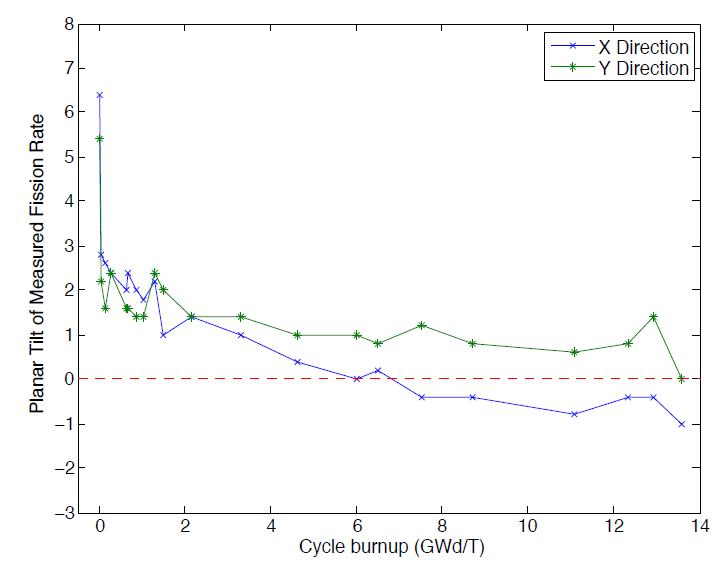
\includegraphics[width=5.0in]{expdata/figs/tilt_cycle1.png}
  \caption{Planar tilt for cycle 1
  \label{fig:cyc_1_tilt}}
\end{figure}

\begin{figure}[hbtp]
  \centering
  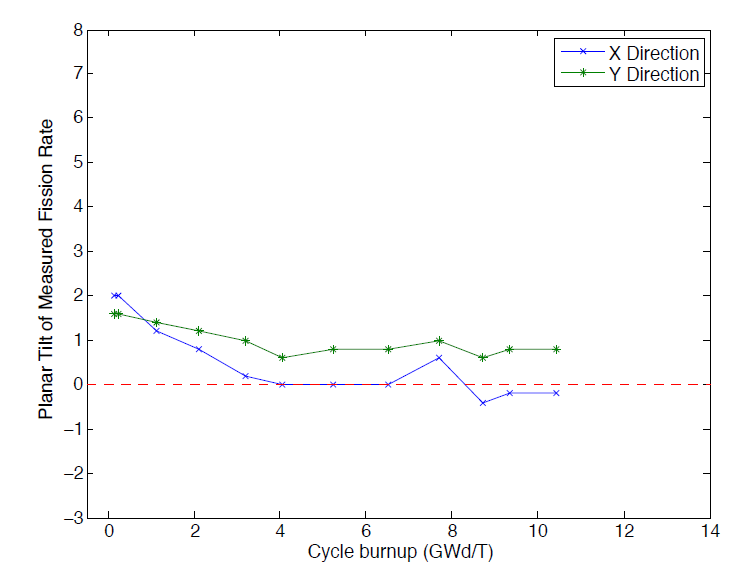
\includegraphics[width=5.0in]{expdata/figs/tilt_cycle2.png}
  \caption{Planar tilt for cycle 2
  \label{fig:cyc_2_tilt}}
\end{figure}

For each burnup, tilt-corrected data at each assembly, as well as tilt-corrected radial 
maps are all available on the {\color{blue}\href{http://crpg.mit.edu/pub/beavrs}{MIT-CRPG website}}. It must be noted that there is no 
definitive explanation for why this tilt in the data arises or the validity of the 
planar tilt correction, so this data should be utilized at the user's own discretion.

\subsubsection{Boron Letdown Curve}
\label{sec:boron_letdown}
Also available is the boron letdown curve during Cycle 1 and Cycle 2 operation.
Figure \ref{fig:boron_letdown} and corresponding Table \ref{tab:boron_letdown}
present the boron letdown data. Finally, the power history reference from
\ac{BOC} for Cycle 1 operation is presented in Figure \ref{fig:power_historyc1}.
Power history data is also available online at the
{\color{blue}\href{http://crpg.mit.edu/pub/beavrs}{MIT-CRPG website}}. In Figure
\ref{fig:power_historyc1}, locations of where detector maps are available are
also shown. Note, the powers shown in Figure \ref{fig:power_historyc1} are 24-hr
averages, whereas, in detector measurement files, powers reported are
instantaneous at the time of measurement. In the plot they are shown to be
coincident with the power history, however, in the files they may be slightly
different. Similarly, Figure \ref{fig:power_historyc2} shows the power history
of Cycle 2.

\begin{figure}[htb]
  \centering
  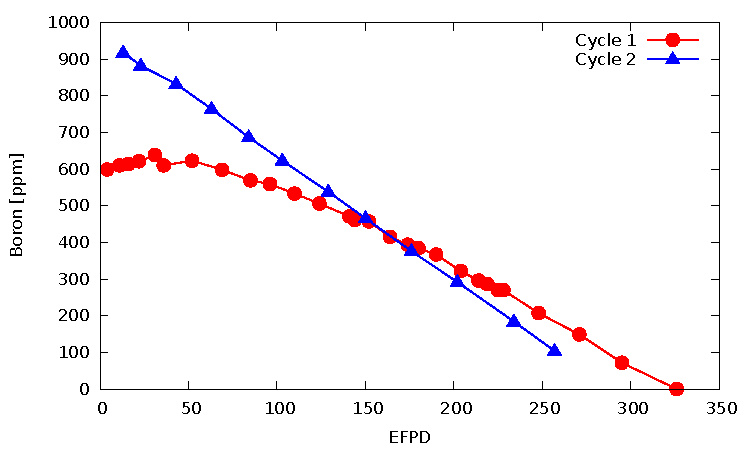
\includegraphics[width=5.5in]{expdata/figs/boron_letdown.pdf}
  \caption{Measured boron letdown curves for two cycles of operation.
  \label{fig:boron_letdown}}
\end{figure}

\begin{table}[htp]
  \centering
  \caption{Boron Letdown Curve Data for Cycles 1 and 2.\label{tab:boron_letdown}}
  \begin{tabular}{l c l c}
    \toprule
    \multicolumn{2}{c}{Cycle 1} &
    \multicolumn{2}{c}{Cycle 2}\\
    \midrule
    \midrule
    \acs{EFPD} & Boron [\acs{ppm}] &  \acs{EFPD} & Boron [\acs{ppm}] \\
    4  & 599 & 13 & 918 \\
    11 & 610 & 23 & 882 \\
    16 & 614 & 43 & 832 \\
    22 & 621 & 63 & 764 \\
    31 & 638 & 84 & 687 \\
    36 & 610 & 103 & 623 \\
    52 & 623 & 129 & 538 \\
    69 & 598 & 150 & 466 \\
    85 & 569 & 176 & 376 \\
    96 & 559 & 202 & 292 \\
   110 & 533 & 234 & 184 \\
   124 & 506 & 257 & 104 \\
   141 & 471 & & \\
   144 & 461 & & \\ 
   152 & 457 &  & \\
   164 & 415 &  & \\
   174 & 394 &  & \\
   177 & 384 &  & \\
   180 & 384 &  & \\
   190 & 367 &  & \\
   204 & 322 &  & \\
   214 & 296 &  & \\
   219 & 286 &  & \\
   225 & 270 &  & \\
   228 & 270 &  & \\
   248 & 207 & & \\
   271 & 149 &  & \\
   295 & 72 &  & \\
   326 & 0 &  & \\
   \bottomrule
  \end{tabular}
\end{table} 
\clearpage
\begin{landscape}
\begin{figure}[htb]
  \centering
  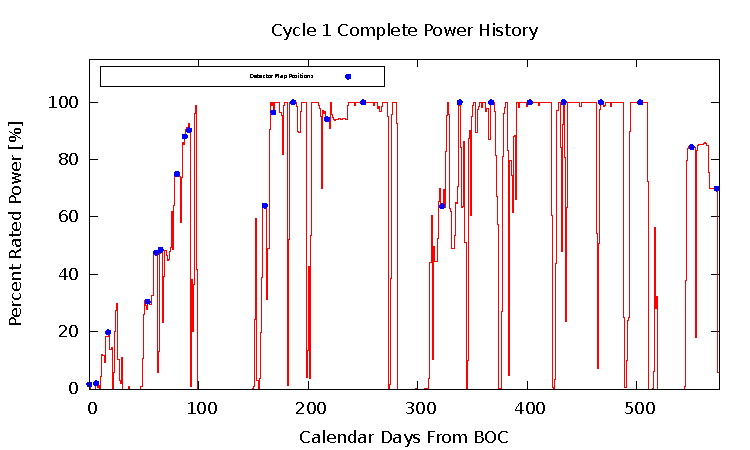
\includegraphics[scale=1.8]{expdata/figs/cycle1.pdf}
  \caption{Power history of Cycle 1.
  \label{fig:power_historyc1}}
\end{figure}
\end{landscape}
\clearpage
\begin{landscape}
\begin{figure}[htb]
  \centering
  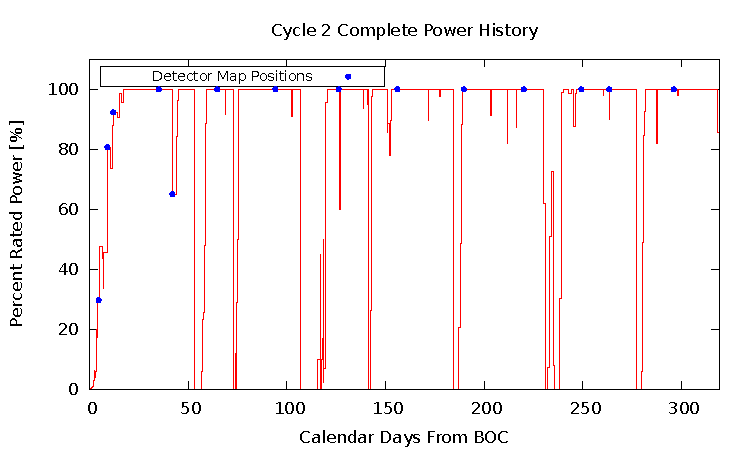
\includegraphics[scale=1.8]{expdata/figs/cycle2.pdf}
  \caption{Power history of Cycle 2.
  \label{fig:power_historyc2}}
\end{figure}
\end{landscape}

%Additional data collected, listed in Table \ref{tab:operdata}
%shows how inlet temperature, critical boron
%concentration, bank D rod position and percent of full power as 
%a function of exposure for cycle 1.
%
%\begin{table}
%  \centering
%  \label{tab:operdata}
%  \caption{Core operating data as a function of exposure}
%  \begin{tabular}{c c c c c c}
%  \toprule
%  Exporsure (EFPD) &  Boron (ppm) & Inlet Temp. (F) & Bank D &  \% Power \\
%  \midrule
%  \midrule
%   .00 &  709 &  559.2 &  212 &   48.6 \\
%  6.00 &  674 &  559.2 &  212 &   48.6 \\
% 21.00 &  609 &  561.1 &  217 &   89.5 \\
% 25.00 &  598 &  561.5 &  207 &   98.5 \\
% 36.00 &  596 &  561.6 &  198 &   99.8 \\
% 52.00 &  590 &  561.6 &  228 &  100.0 \\
% 80.00 &  556 &  561.3 &  195 &   94.0 \\
%110.00 &  494 &  561.6 &  193 &  100.0 \\
%140.00 &  437 &  561.6 &  208 &  100.0 \\
%144.00 &  476 &  559.9 &  178 &   64.0 \\
%150.00 &  416 &  561.6 &  199 &  100.0 \\
%156.00 &  404 &  561.6 &  199 &  100.0 \\
%180.00 &  352 &  561.6 &  215 &  100.0 \\
%220.00 &  258 &  561.6 &  223 &  100.0 \\
%235.00 &  218 &  561.6 &  208 &  100.0 \\
%266.00 &  140 &  561.6 &  217 &  100.0 \\
%296.00 &   58 &  561.6 &  215 &  100.0 \\
%310.00 &   49 &  560.9 &  216 &   84.5 \\
%326.00 &   31 &  560.2 &  208 &   70.0 \\
%327.00 &   29 &  560.2 &  208 &   70.0 \\
%  \bottomrule
%  \end{tabular}
%\end{table}

%%%%%%%%%%%%%%%%%%%%%%%%%%%%%%%%%%%%%%%%%%%%%%%%%%%%%%%%%%%%%%%%%%%%%%%%%%%%%%%%
\subsection{Uncertainty Quantification of Measurements}
\label{sec:uq_measurements}

In addition to the model parameters and measured data, the associated uncertainties
are also essential for the validation of high-fidelity tools.
A series of uncertainty quantification work has been carried out in the BEAVRS
benchmark. Uncertainties of various measurements are available in the data package,
while the evaluation methods are detailed in \cite{liang2017uq_beavrs} and \cite{kumar2018final_report}.
